\documentclass[twoside]{book}

% Packages required by doxygen
\usepackage{calc}
\usepackage{doxygen}
\usepackage{graphicx}
\usepackage[utf8]{inputenc}
\usepackage{makeidx}
\usepackage{multicol}
\usepackage{multirow}
\usepackage{textcomp}
\usepackage[table]{xcolor}

% Font selection
\usepackage[T1]{fontenc}
\usepackage{mathptmx}
\usepackage[scaled=.90]{helvet}
\usepackage{courier}
\usepackage{amssymb}
\usepackage{sectsty}
\renewcommand{\familydefault}{\sfdefault}
\allsectionsfont{%
  \fontseries{bc}\selectfont%
  \color{darkgray}%
}
\renewcommand{\DoxyLabelFont}{%
  \fontseries{bc}\selectfont%
  \color{darkgray}%
}

% Page & text layout
\usepackage{geometry}
\geometry{%
  a4paper,%
  top=2.5cm,%
  bottom=2.5cm,%
  left=2.5cm,%
  right=2.5cm%
}
\tolerance=750
\hfuzz=15pt
\hbadness=750
\setlength{\emergencystretch}{15pt}
\setlength{\parindent}{0cm}
\setlength{\parskip}{0.2cm}
\makeatletter
\renewcommand{\paragraph}{%
  \@startsection{paragraph}{4}{0ex}{-1.0ex}{1.0ex}{%
    \normalfont\normalsize\bfseries\SS@parafont%
  }%
}
\renewcommand{\subparagraph}{%
  \@startsection{subparagraph}{5}{0ex}{-1.0ex}{1.0ex}{%
    \normalfont\normalsize\bfseries\SS@subparafont%
  }%
}
\makeatother

% Headers & footers
\usepackage{fancyhdr}
\pagestyle{fancyplain}
\fancyhead[LE]{\fancyplain{}{\bfseries\thepage}}
\fancyhead[CE]{\fancyplain{}{}}
\fancyhead[RE]{\fancyplain{}{\bfseries\leftmark}}
\fancyhead[LO]{\fancyplain{}{\bfseries\rightmark}}
\fancyhead[CO]{\fancyplain{}{}}
\fancyhead[RO]{\fancyplain{}{\bfseries\thepage}}
\fancyfoot[LE]{\fancyplain{}{}}
\fancyfoot[CE]{\fancyplain{}{}}
\fancyfoot[RE]{\fancyplain{}{\bfseries\scriptsize Generated on Thu Dec 14 2017 08\-:04\-:03 for tmxparser by Doxygen }}
\fancyfoot[LO]{\fancyplain{}{\bfseries\scriptsize Generated on Thu Dec 14 2017 08\-:04\-:03 for tmxparser by Doxygen }}
\fancyfoot[CO]{\fancyplain{}{}}
\fancyfoot[RO]{\fancyplain{}{}}
\renewcommand{\footrulewidth}{0.4pt}
\renewcommand{\chaptermark}[1]{%
  \markboth{#1}{}%
}
\renewcommand{\sectionmark}[1]{%
  \markright{\thesection\ #1}%
}

% Indices & bibliography
\usepackage{natbib}
\usepackage[titles]{tocloft}
\setcounter{tocdepth}{3}
\setcounter{secnumdepth}{5}
\makeindex

% Hyperlinks (required, but should be loaded last)
\usepackage{ifpdf}
\ifpdf
  \usepackage[pdftex,pagebackref=true]{hyperref}
\else
  \usepackage[ps2pdf,pagebackref=true]{hyperref}
\fi
\hypersetup{%
  colorlinks=true,%
  linkcolor=blue,%
  citecolor=blue,%
  unicode%
}

% Custom commands
\newcommand{\clearemptydoublepage}{%
  \newpage{\pagestyle{empty}\cleardoublepage}%
}


%===== C O N T E N T S =====

\begin{document}

% Titlepage & ToC
\hypersetup{pageanchor=false}
\pagenumbering{roman}
\begin{titlepage}
\vspace*{7cm}
\begin{center}%
{\Large tmxparser \\[1ex]\large 2.\-1.\-0 }\\
\vspace*{1cm}
{\large Generated by Doxygen 1.8.6}\\
\vspace*{0.5cm}
{\small Thu Dec 14 2017 08:04:03}\\
\end{center}
\end{titlepage}
\clearemptydoublepage
\tableofcontents
\clearemptydoublepage
\pagenumbering{arabic}
\hypersetup{pageanchor=true}

%--- Begin generated contents ---
\chapter{Main Page}
\label{index}\hypertarget{index}{}\href{https://travis-ci.org/sainteos/tmxparser}{\tt !\mbox{[}Build Status\mbox{]}(https\-://travis-\/ci.\-org/sainteos/tmxparser.\-svg?branch=master)}

This is a library for parsing the maps generated by \href{https://github.com/bjorn/tiled/}{\tt Tiled Map Editor}.

The T\-M\-X format is based upon X\-M\-L and may contain compressed and encoded tile data to save memory and reduce file sizes. This parser uses the \href{http://www.grinninglizard.com/tinyxml/}{\tt Tiny\-X\-M\-L} library and its D\-O\-M interface to parse T\-M\-X files.

An example file is provided to understand how to use the library.

This project is forked from \href{https://code.google.com/p/tmx-parser/}{\tt https\-://code.\-google.\-com/p/tmx-\/parser/} because\-:


\begin{DoxyItemize}
\item Organized cleanly for inclusion into Debian. This means depending on zlib and Tiny\-X\-M\-L externally, building a shared library, installing to the correct prefix, etc.
\item Drop support for Android and Windows. If you want a Windows build, use \href{https://github.com/mxe/mxe}{\tt mxe}.
\item Resolving the open issues\-: \href{https://code.google.com/p/tmx-parser/issues/list}{\tt https\-://code.\-google.\-com/p/tmx-\/parser/issues/list}
\item More robust tests.
\end{DoxyItemize}

\subsection*{Features}


\begin{DoxyItemize}
\item Conformity with the \href{http://doc.mapeditor.org/en/latest/reference/tmx-map-format/}{\tt T\-M\-X specification page}.
\item Decodes and decompresses tile data.
\item Can parse properties as both integers, real numbers and literals (strings).
\item Can parse the map file when stored in memory.
\item Does not rely on any graphics library.
\item Animated tile support.
\end{DoxyItemize}

\subsection*{Dependencies}


\begin{DoxyItemize}
\item zlib
\item Tiny\-X\-M\-L
\end{DoxyItemize}

\subsection*{Installation}

``` mkdir build cd build cmake .. make sudo make install ``` 
\chapter{Changelog}
\label{md__home_travis_build_sainteos_tmxparser_CHANGELOG}
\hypertarget{md__home_travis_build_sainteos_tmxparser_CHANGELOG}{}
\subsubsection*{Next release}


\begin{DoxyItemize}
\item georgerbr\-:
\begin{DoxyItemize}
\item Make tileset parsing not depend on optional attrs of $<$image$>$
\end{DoxyItemize}
\item Andrew Kelley\-:
\begin{DoxyItemize}
\item Add Find\-Tmx\-Parser.\-cmake example
\end{DoxyItemize}
\item Wasabi2007\-:
\begin{DoxyItemize}
\item Added support for Collision Tiles
\item Changed data format in Point from int to float to follow Tiled format (bugfix)
\end{DoxyItemize}
\item Acedio\-:
\begin{DoxyItemize}
\item Adding missing library dependencies to Tmx\-Util.\-cpp
\end{DoxyItemize}
\item Tigran Saluev\-:
\begin{DoxyItemize}
\item Add support for $<$image$>$ in $<$tile$>$
\end{DoxyItemize}
\item Richel Bilderbeek\-:
\begin{DoxyItemize}
\item Removed const return types
\end{DoxyItemize}
\item Blazej Floch\-:
\begin{DoxyItemize}
\item Small changes to Tmx\-Property\-Set
\item Better compatibility with cmake project as subdirectory
\end{DoxyItemize}
\item Tamir Atias\-:
\begin{DoxyItemize}
\item Add support for typed properties (added in Tiled 0.\-16)
\end{DoxyItemize}
\item Peter Asplund (Az\-P)\-:
\begin{DoxyItemize}
\item Add C++11 requirement in C\-Make\-Lists.\-txt
\end{DoxyItemize}
\item Solever Lee\-:
\begin{DoxyItemize}
\item added 'tilecount' and 'columns' properity for 'tileset' element
\end{DoxyItemize}
\item Guillaume Bertholon (Sakarah)\-:
\begin{DoxyItemize}
\item Add support for color and file property types (added in Tiled 0.\-17)
\item Add Doxygen documentation
\end{DoxyItemize}
\item Tardo\-:
\begin{DoxyItemize}
\item Get tile by index
\end{DoxyItemize}
\end{DoxyItemize}

\subsubsection*{2.\-0.\-1}


\begin{DoxyItemize}
\item georgerbr\-:
\begin{DoxyItemize}
\item Fix incorrect version number reported.
\end{DoxyItemize}
\end{DoxyItemize}

\subsubsection*{2.\-0.\-0}


\begin{DoxyItemize}
\item georgerbr\-:
\begin{DoxyItemize}
\item Fix \#9, \#13 and \#17
\item Implement missing elements (except T\-S\-X loading) from T\-M\-X format
\item Initialize tile\-Offset to N\-U\-L\-L in \hyperlink{classTmx_1_1Tileset}{Tmx\-::\-Tileset}.
\item Corrected misspelled attribute name.
\item Catch up to T\-M\-X Format as of Tiled 0.\-12
\end{DoxyItemize}
\item Alessio Linares\-:
\begin{DoxyItemize}
\item fixed gid of Map\-Tile being local to its tileset and not global
\item Added getter for the id of an object
\item Added getter for the nextobjectid map parameter
\item Added version defines (minor and major)
\item Changes commented on commit b5e6040
\end{DoxyItemize}
\item Thomas Fischer\-:
\begin{DoxyItemize}
\item fixed a trim function that was messing with the underlying string
\item enabled loading of external tileset (T\-S\-X) files
\item fixed naming convention
\item replaced the long file open routine with a tinyxml load\-File call
\end{DoxyItemize}
\item Ashley Davis (Sgt\-Co\-D\-Fish)\-:
\begin{DoxyItemize}
\item Update gitignore, A\-U\-T\-H\-O\-R\-S
\item Add support for loading and storing animated tiles, mostly in \hyperlink{TmxTile_8h_source}{Tmx\-Tile.\-h}/cpp.
\item Add example animated tileset and update example.\-tmx to include an animated example.
\end{DoxyItemize}
\item Andrew Kelley\-:
\begin{DoxyItemize}
\item better Tmx\-Property\-Set A\-P\-I
\end{DoxyItemize}
\item Vincent Heuken\-:
\begin{DoxyItemize}
\item added {\ttfamily U\-S\-E\-\_\-\-M\-I\-N\-I\-Z} option
\end{DoxyItemize}
\item Ashley Davis\-:
\begin{DoxyItemize}
\item Fix formatting and incorrect method name in \hyperlink{TmxTile_8h_source}{Tmx\-Tile.\-h}, Tmx\-Tile.\-cpp and test.\-cpp
\end{DoxyItemize}
\item Edward Lu\-:
\begin{DoxyItemize}
\item Add rotation property on objects
\end{DoxyItemize}
\item Jamie Nicol\-:
\begin{DoxyItemize}
\item Add pkg-\/config file.
\end{DoxyItemize}
\item Kris Mc\-Aulay\-:
\begin{DoxyItemize}
\item Modified the cmake file to look for tinyxml2
\end{DoxyItemize}
\item krux02\-:
\begin{DoxyItemize}
\item Update C\-Make\-Lists.\-txt
\end{DoxyItemize}
\end{DoxyItemize}

\subsubsection*{1.\-0.\-0}


\begin{DoxyItemize}
\item Initial fork from \href{https://code.google.com/p/tmx-parser/}{\tt https\-://code.\-google.\-com/p/tmx-\/parser/}
\item Layer\-: Add getters for opacity and visible
\item Drop support for Android and Windows. If you want a Windows build, use mxe.
\item Build\-: Create and install a shared library in addition to a static object.
\item Build\-: Depend on system zlib and Tiny\-X\-M\-L.
\item Drop {\ttfamily U\-S\-E\-\_\-\-S\-D\-L2\-\_\-\-L\-O\-A\-D} support. 
\end{DoxyItemize}
\chapter{Hierarchical Index}
\section{Class Hierarchy}
This inheritance list is sorted roughly, but not completely, alphabetically\-:\begin{DoxyCompactList}
\item \contentsline{section}{Tmx\-:\-:Animation\-Frame}{\pageref{classTmx_1_1AnimationFrame}}{}
\item \contentsline{section}{Tmx\-:\-:Color}{\pageref{classTmx_1_1Color}}{}
\item \contentsline{section}{Tmx\-:\-:Ellipse}{\pageref{classTmx_1_1Ellipse}}{}
\item \contentsline{section}{Tmx\-:\-:Image}{\pageref{classTmx_1_1Image}}{}
\item \contentsline{section}{Tmx\-:\-:Layer}{\pageref{classTmx_1_1Layer}}{}
\begin{DoxyCompactList}
\item \contentsline{section}{Tmx\-:\-:Image\-Layer}{\pageref{classTmx_1_1ImageLayer}}{}
\item \contentsline{section}{Tmx\-:\-:Object\-Group}{\pageref{classTmx_1_1ObjectGroup}}{}
\item \contentsline{section}{Tmx\-:\-:Tile\-Layer}{\pageref{classTmx_1_1TileLayer}}{}
\end{DoxyCompactList}
\item \contentsline{section}{Tmx\-:\-:Map}{\pageref{classTmx_1_1Map}}{}
\item \contentsline{section}{Tmx\-:\-:Map\-Tile}{\pageref{structTmx_1_1MapTile}}{}
\item \contentsline{section}{Tmx\-:\-:Object}{\pageref{classTmx_1_1Object}}{}
\item \contentsline{section}{Tmx\-:\-:Point}{\pageref{structTmx_1_1Point}}{}
\item \contentsline{section}{Tmx\-:\-:Polygon}{\pageref{classTmx_1_1Polygon}}{}
\item \contentsline{section}{Tmx\-:\-:Polyline}{\pageref{classTmx_1_1Polyline}}{}
\item \contentsline{section}{Tmx\-:\-:Property}{\pageref{classTmx_1_1Property}}{}
\item \contentsline{section}{Tmx\-:\-:Property\-Set}{\pageref{classTmx_1_1PropertySet}}{}
\item \contentsline{section}{Tmx\-:\-:Terrain}{\pageref{classTmx_1_1Terrain}}{}
\item \contentsline{section}{Tmx\-:\-:Terrain\-Array}{\pageref{classTmx_1_1TerrainArray}}{}
\item \contentsline{section}{Tmx\-:\-:Tile}{\pageref{classTmx_1_1Tile}}{}
\item \contentsline{section}{Tmx\-:\-:Tile\-Offset}{\pageref{classTmx_1_1TileOffset}}{}
\item \contentsline{section}{Tmx\-:\-:Tileset}{\pageref{classTmx_1_1Tileset}}{}
\end{DoxyCompactList}

\chapter{Class Index}
\section{Class List}
Here are the classes, structs, unions and interfaces with brief descriptions\-:\begin{DoxyCompactList}
\item\contentsline{section}{\hyperlink{classTmx_1_1AnimationFrame}{Tmx\-::\-Animation\-Frame} \\*Class containing information about an animated tile }{\pageref{classTmx_1_1AnimationFrame}}{}
\item\contentsline{section}{\hyperlink{classTmx_1_1Color}{Tmx\-::\-Color} \\*A class used for storing information about a color }{\pageref{classTmx_1_1Color}}{}
\item\contentsline{section}{\hyperlink{classTmx_1_1Ellipse}{Tmx\-::\-Ellipse} \\*Class to store an \hyperlink{classTmx_1_1Ellipse}{Ellipse} of an \hyperlink{classTmx_1_1Object}{Object} }{\pageref{classTmx_1_1Ellipse}}{}
\item\contentsline{section}{\hyperlink{classTmx_1_1Image}{Tmx\-::\-Image} \\*A class used for storing information about an image within a tileset }{\pageref{classTmx_1_1Image}}{}
\item\contentsline{section}{\hyperlink{classTmx_1_1ImageLayer}{Tmx\-::\-Image\-Layer} \\*A class used for holding information about a background image }{\pageref{classTmx_1_1ImageLayer}}{}
\item\contentsline{section}{\hyperlink{classTmx_1_1Layer}{Tmx\-::\-Layer} \\*Base class for other layer types }{\pageref{classTmx_1_1Layer}}{}
\item\contentsline{section}{\hyperlink{classTmx_1_1Map}{Tmx\-::\-Map} \\*This class is the root class of the parser }{\pageref{classTmx_1_1Map}}{}
\item\contentsline{section}{\hyperlink{structTmx_1_1MapTile}{Tmx\-::\-Map\-Tile} \\*Struct to store information about a specific tile in the map layer }{\pageref{structTmx_1_1MapTile}}{}
\item\contentsline{section}{\hyperlink{classTmx_1_1Object}{Tmx\-::\-Object} \\*Class used for representing a single object from the objectgroup }{\pageref{classTmx_1_1Object}}{}
\item\contentsline{section}{\hyperlink{classTmx_1_1ObjectGroup}{Tmx\-::\-Object\-Group} \\*A class used for holding a list of objects }{\pageref{classTmx_1_1ObjectGroup}}{}
\item\contentsline{section}{\hyperlink{structTmx_1_1Point}{Tmx\-::\-Point} \\*Used to store a vertex of a Polygon/\-Polyline }{\pageref{structTmx_1_1Point}}{}
\item\contentsline{section}{\hyperlink{classTmx_1_1Polygon}{Tmx\-::\-Polygon} \\*Class to store a \hyperlink{classTmx_1_1Polygon}{Polygon} of an \hyperlink{classTmx_1_1Object}{Object} }{\pageref{classTmx_1_1Polygon}}{}
\item\contentsline{section}{\hyperlink{classTmx_1_1Polyline}{Tmx\-::\-Polyline} \\*Class to store a \hyperlink{classTmx_1_1Polyline}{Polyline} of an \hyperlink{classTmx_1_1Object}{Object} }{\pageref{classTmx_1_1Polyline}}{}
\item\contentsline{section}{\hyperlink{classTmx_1_1Property}{Tmx\-::\-Property} \\*Used to store a (typed) property }{\pageref{classTmx_1_1Property}}{}
\item\contentsline{section}{\hyperlink{classTmx_1_1PropertySet}{Tmx\-::\-Property\-Set} \\*This class contains a map of properties }{\pageref{classTmx_1_1PropertySet}}{}
\item\contentsline{section}{\hyperlink{classTmx_1_1Terrain}{Tmx\-::\-Terrain} \\*Class to contain information about every terrain in the tileset/terraintypes element }{\pageref{classTmx_1_1Terrain}}{}
\item\contentsline{section}{\hyperlink{classTmx_1_1TerrainArray}{Tmx\-::\-Terrain\-Array} \\*Class to parse terrain types, which can be referenced from the terrain attribute of the tileset/tile element }{\pageref{classTmx_1_1TerrainArray}}{}
\item\contentsline{section}{\hyperlink{classTmx_1_1Tile}{Tmx\-::\-Tile} \\*Class to contain information about every tile in the tileset/tiles element }{\pageref{classTmx_1_1Tile}}{}
\item\contentsline{section}{\hyperlink{classTmx_1_1TileLayer}{Tmx\-::\-Tile\-Layer} \\*Used for storing information about the tile ids for every tile layer }{\pageref{classTmx_1_1TileLayer}}{}
\item\contentsline{section}{\hyperlink{classTmx_1_1TileOffset}{Tmx\-::\-Tile\-Offset} \\*A class used for used to specify an offset in pixels, to be applied when drawing a tile from the related tileset }{\pageref{classTmx_1_1TileOffset}}{}
\item\contentsline{section}{\hyperlink{classTmx_1_1Tileset}{Tmx\-::\-Tileset} \\*A class used for storing information about each of the tilesets }{\pageref{classTmx_1_1Tileset}}{}
\end{DoxyCompactList}

\chapter{Class Documentation}
\hypertarget{classTmx_1_1AnimationFrame}{\section{Tmx\-:\-:Animation\-Frame Class Reference}
\label{classTmx_1_1AnimationFrame}\index{Tmx\-::\-Animation\-Frame@{Tmx\-::\-Animation\-Frame}}
}


Class containing information about an animated tile.  




{\ttfamily \#include $<$Tmx\-Tile.\-h$>$}

\subsection*{Public Member Functions}
\begin{DoxyCompactItemize}
\item 
\hypertarget{classTmx_1_1AnimationFrame_a5c82aebb547d7e1131d3189978900040}{\hyperlink{classTmx_1_1AnimationFrame_a5c82aebb547d7e1131d3189978900040}{Animation\-Frame} ()}\label{classTmx_1_1AnimationFrame_a5c82aebb547d7e1131d3189978900040}

\begin{DoxyCompactList}\small\item\em This constructor shouldn't be used, ideally. \end{DoxyCompactList}\item 
\hypertarget{classTmx_1_1AnimationFrame_a84a24bfb968c6e8c37e2031acbaf8df4}{\hyperlink{classTmx_1_1AnimationFrame_a84a24bfb968c6e8c37e2031acbaf8df4}{Animation\-Frame} (int tile\-I\-D, unsigned int duration)}\label{classTmx_1_1AnimationFrame_a84a24bfb968c6e8c37e2031acbaf8df4}

\begin{DoxyCompactList}\small\item\em Create a new animation frame with a specified tile id and duration. \end{DoxyCompactList}\item 
\hypertarget{classTmx_1_1AnimationFrame_ae55cf73d125a551f130dca4d04740193}{int \hyperlink{classTmx_1_1AnimationFrame_ae55cf73d125a551f130dca4d04740193}{Get\-Tile\-I\-D} () const }\label{classTmx_1_1AnimationFrame_ae55cf73d125a551f130dca4d04740193}

\begin{DoxyCompactList}\small\item\em Get the tile id of this frame, relative to the containing tileset. \end{DoxyCompactList}\item 
\hypertarget{classTmx_1_1AnimationFrame_a50c2a730e35796dd20af47398bdd9941}{unsigned int \hyperlink{classTmx_1_1AnimationFrame_a50c2a730e35796dd20af47398bdd9941}{Get\-Duration} () const }\label{classTmx_1_1AnimationFrame_a50c2a730e35796dd20af47398bdd9941}

\begin{DoxyCompactList}\small\item\em Get the duration of this frame in milliseconds. \end{DoxyCompactList}\end{DoxyCompactItemize}


\subsection{Detailed Description}
Class containing information about an animated tile. 

This includes the duration of each frame and the various ids of each frame in the animation. 

The documentation for this class was generated from the following file\-:\begin{DoxyCompactItemize}
\item 
/home/travis/build/sainteos/tmxparser/src/Tmx\-Tile.\-h\end{DoxyCompactItemize}

\hypertarget{classTmx_1_1Color}{\section{Tmx\-:\-:Color Class Reference}
\label{classTmx_1_1Color}\index{Tmx\-::\-Color@{Tmx\-::\-Color}}
}


A class used for storing information about a color.  




{\ttfamily \#include $<$Tmx\-Color.\-h$>$}

\subsection*{Public Member Functions}
\begin{DoxyCompactItemize}
\item 
\hypertarget{classTmx_1_1Color_ac462194348bb366f3b90d872d18486e2}{\hyperlink{classTmx_1_1Color_ac462194348bb366f3b90d872d18486e2}{Color} ()}\label{classTmx_1_1Color_ac462194348bb366f3b90d872d18486e2}

\begin{DoxyCompactList}\small\item\em Default constructor for a fully transparent black color. \end{DoxyCompactList}\item 
\hypertarget{classTmx_1_1Color_a29e71f2f41c56cbd07369f0d4c2e9531}{\hyperlink{classTmx_1_1Color_a29e71f2f41c56cbd07369f0d4c2e9531}{Color} (uint32\-\_\-t color)}\label{classTmx_1_1Color_a29e71f2f41c56cbd07369f0d4c2e9531}

\begin{DoxyCompactList}\small\item\em Initialize the color with a 32 bit A\-R\-G\-B representation. \end{DoxyCompactList}\item 
\hypertarget{classTmx_1_1Color_ac2bfcd16e5a09544dc78de7e0bdda14e}{\hyperlink{classTmx_1_1Color_ac2bfcd16e5a09544dc78de7e0bdda14e}{Color} (uint8\-\_\-t r, uint8\-\_\-t g, uint8\-\_\-t b, uint8\-\_\-t a=255)}\label{classTmx_1_1Color_ac2bfcd16e5a09544dc78de7e0bdda14e}

\begin{DoxyCompactList}\small\item\em Initialize the color with a red, green, blue and optionally alpha values. \end{DoxyCompactList}\item 
\hypertarget{classTmx_1_1Color_a46358ffd46a11af3a7d6a01aee9a4d08}{\hyperlink{classTmx_1_1Color_a46358ffd46a11af3a7d6a01aee9a4d08}{Color} (const std\-::string \&str)}\label{classTmx_1_1Color_a46358ffd46a11af3a7d6a01aee9a4d08}

\begin{DoxyCompactList}\small\item\em Initialize a color from a string hexadecimal representation in the format \char`\"{}\#\-A\-A\-R\-R\-G\-G\-B\-B\char`\"{} or \char`\"{}\#\-R\-R\-G\-G\-B\-B\char`\"{}. \end{DoxyCompactList}\item 
\hypertarget{classTmx_1_1Color_a47a6ba4d9445bcdcafefc63f41c46d69}{\hyperlink{classTmx_1_1Color_a47a6ba4d9445bcdcafefc63f41c46d69}{Color} (const \hyperlink{classTmx_1_1Color}{Color} \&)=default}\label{classTmx_1_1Color_a47a6ba4d9445bcdcafefc63f41c46d69}

\begin{DoxyCompactList}\small\item\em Default copy constructor. \end{DoxyCompactList}\item 
\hypertarget{classTmx_1_1Color_ac3b6cab5ff3052ff7253d70fc0ecba50}{\hyperlink{classTmx_1_1Color}{Color} \& \hyperlink{classTmx_1_1Color_ac3b6cab5ff3052ff7253d70fc0ecba50}{operator=} (const \hyperlink{classTmx_1_1Color}{Color} \&)=default}\label{classTmx_1_1Color_ac3b6cab5ff3052ff7253d70fc0ecba50}

\begin{DoxyCompactList}\small\item\em Default asignment operator. \end{DoxyCompactList}\item 
\hypertarget{classTmx_1_1Color_a7514ffb5992a35369655c2ca5e873012}{bool \hyperlink{classTmx_1_1Color_a7514ffb5992a35369655c2ca5e873012}{operator==} (const \hyperlink{classTmx_1_1Color}{Color} \&o)}\label{classTmx_1_1Color_a7514ffb5992a35369655c2ca5e873012}

\begin{DoxyCompactList}\small\item\em Check if two colors have the exact same four components. \end{DoxyCompactList}\item 
\hypertarget{classTmx_1_1Color_a82c3e3199f93d1ce9c2babadd6a9bf40}{bool \hyperlink{classTmx_1_1Color_a82c3e3199f93d1ce9c2babadd6a9bf40}{operator!=} (const \hyperlink{classTmx_1_1Color}{Color} \&o)}\label{classTmx_1_1Color_a82c3e3199f93d1ce9c2babadd6a9bf40}

\begin{DoxyCompactList}\small\item\em Check if two colors are different. \end{DoxyCompactList}\item 
\hypertarget{classTmx_1_1Color_a69661b363a65a82ccecf42209e4ca366}{uint8\-\_\-t \hyperlink{classTmx_1_1Color_a69661b363a65a82ccecf42209e4ca366}{Get\-Alpha} () const }\label{classTmx_1_1Color_a69661b363a65a82ccecf42209e4ca366}

\begin{DoxyCompactList}\small\item\em Get the alpha component of the color. \end{DoxyCompactList}\item 
\hypertarget{classTmx_1_1Color_ac188b64dda182848df9469ee549bb26a}{uint8\-\_\-t \hyperlink{classTmx_1_1Color_ac188b64dda182848df9469ee549bb26a}{Get\-Red} () const }\label{classTmx_1_1Color_ac188b64dda182848df9469ee549bb26a}

\begin{DoxyCompactList}\small\item\em Get the red component of the color. \end{DoxyCompactList}\item 
\hypertarget{classTmx_1_1Color_a82a3f08a25d58d2d2f244a8347cf0bce}{uint8\-\_\-t \hyperlink{classTmx_1_1Color_a82a3f08a25d58d2d2f244a8347cf0bce}{Get\-Green} () const }\label{classTmx_1_1Color_a82a3f08a25d58d2d2f244a8347cf0bce}

\begin{DoxyCompactList}\small\item\em Get the green component of the color. \end{DoxyCompactList}\item 
\hypertarget{classTmx_1_1Color_ab3dd06474d6403dbf9bd6bcd0d28a70a}{uint8\-\_\-t \hyperlink{classTmx_1_1Color_ab3dd06474d6403dbf9bd6bcd0d28a70a}{Get\-Blue} () const }\label{classTmx_1_1Color_ab3dd06474d6403dbf9bd6bcd0d28a70a}

\begin{DoxyCompactList}\small\item\em Get the blue component of the color. \end{DoxyCompactList}\item 
\hypertarget{classTmx_1_1Color_aed77854b09267887bd289f4622e831d1}{bool \hyperlink{classTmx_1_1Color_aed77854b09267887bd289f4622e831d1}{Is\-Transparent} () const }\label{classTmx_1_1Color_aed77854b09267887bd289f4622e831d1}

\begin{DoxyCompactList}\small\item\em Return true if the color is fully transparent (ie alpha value is 0). \end{DoxyCompactList}\item 
\hypertarget{classTmx_1_1Color_a20ae331f91f72ca3db0068508a7b0317}{uint32\-\_\-t \hyperlink{classTmx_1_1Color_a20ae331f91f72ca3db0068508a7b0317}{To\-Int} () const }\label{classTmx_1_1Color_a20ae331f91f72ca3db0068508a7b0317}

\begin{DoxyCompactList}\small\item\em Get the 32 bits integer representing the color. The 8 highest bits are for the alpha channel, then the red, the green and the blue. \end{DoxyCompactList}\item 
\hypertarget{classTmx_1_1Color_af20cd78adf89d3c3e81ee126e3a8be73}{std\-::string \hyperlink{classTmx_1_1Color_af20cd78adf89d3c3e81ee126e3a8be73}{To\-String} () const }\label{classTmx_1_1Color_af20cd78adf89d3c3e81ee126e3a8be73}

\begin{DoxyCompactList}\small\item\em Get a string representation of the color in the format \char`\"{}\#\-A\-A\-R\-R\-G\-G\-B\-B\char`\"{}. \end{DoxyCompactList}\end{DoxyCompactItemize}


\subsection{Detailed Description}
A class used for storing information about a color. 

The documentation for this class was generated from the following files\-:\begin{DoxyCompactItemize}
\item 
/home/travis/build/sainteos/tmxparser/src/Tmx\-Color.\-h\item 
/home/travis/build/sainteos/tmxparser/src/Tmx\-Color.\-cpp\end{DoxyCompactItemize}

\hypertarget{classTmx_1_1Ellipse}{\section{Tmx\-:\-:Ellipse Class Reference}
\label{classTmx_1_1Ellipse}\index{Tmx\-::\-Ellipse@{Tmx\-::\-Ellipse}}
}


Class to store an \hyperlink{classTmx_1_1Ellipse}{Ellipse} of an \hyperlink{classTmx_1_1Object}{Object}.  




{\ttfamily \#include $<$Tmx\-Ellipse.\-h$>$}

\subsection*{Public Member Functions}
\begin{DoxyCompactItemize}
\item 
\hypertarget{classTmx_1_1Ellipse_a83ab98716ec7cee2925b379c019c4562}{\hyperlink{classTmx_1_1Ellipse_a83ab98716ec7cee2925b379c019c4562}{Ellipse} (int x, int y, int width, int height)}\label{classTmx_1_1Ellipse_a83ab98716ec7cee2925b379c019c4562}

\begin{DoxyCompactList}\small\item\em Construct an ellipse at the given top left position with the given size. \end{DoxyCompactList}\item 
\hypertarget{classTmx_1_1Ellipse_a8e1ef78d1dfba155c27f9964760d4b59}{int \hyperlink{classTmx_1_1Ellipse_a8e1ef78d1dfba155c27f9964760d4b59}{Get\-Center\-X} () const }\label{classTmx_1_1Ellipse_a8e1ef78d1dfba155c27f9964760d4b59}

\begin{DoxyCompactList}\small\item\em Get the center of the object, in pixels. \end{DoxyCompactList}\item 
\hypertarget{classTmx_1_1Ellipse_aaae950d8553312067c6187263c320225}{int \hyperlink{classTmx_1_1Ellipse_aaae950d8553312067c6187263c320225}{Get\-Center\-Y} () const }\label{classTmx_1_1Ellipse_aaae950d8553312067c6187263c320225}

\begin{DoxyCompactList}\small\item\em Get the center of the object, in pixels. \end{DoxyCompactList}\item 
\hypertarget{classTmx_1_1Ellipse_a0bfb57d6097e0c7776303e03abaaebbf}{int \hyperlink{classTmx_1_1Ellipse_a0bfb57d6097e0c7776303e03abaaebbf}{Get\-Radius\-X} () const }\label{classTmx_1_1Ellipse_a0bfb57d6097e0c7776303e03abaaebbf}

\begin{DoxyCompactList}\small\item\em Get the Radius\-X of the object, in pixels. \end{DoxyCompactList}\item 
\hypertarget{classTmx_1_1Ellipse_ac00de47b8ef54f6ef5116c935ebac025}{int \hyperlink{classTmx_1_1Ellipse_ac00de47b8ef54f6ef5116c935ebac025}{Get\-Radius\-Y} () const }\label{classTmx_1_1Ellipse_ac00de47b8ef54f6ef5116c935ebac025}

\begin{DoxyCompactList}\small\item\em Get the Radius\-Y of the object, in pixels. \end{DoxyCompactList}\end{DoxyCompactItemize}


\subsection{Detailed Description}
Class to store an \hyperlink{classTmx_1_1Ellipse}{Ellipse} of an \hyperlink{classTmx_1_1Object}{Object}. 

The documentation for this class was generated from the following files\-:\begin{DoxyCompactItemize}
\item 
/home/travis/build/sainteos/tmxparser/src/Tmx\-Ellipse.\-h\item 
/home/travis/build/sainteos/tmxparser/src/Tmx\-Ellipse.\-cpp\end{DoxyCompactItemize}

\hypertarget{classTmx_1_1Image}{\section{Tmx\-:\-:Image Class Reference}
\label{classTmx_1_1Image}\index{Tmx\-::\-Image@{Tmx\-::\-Image}}
}


A class used for storing information about an image within a tileset.  




{\ttfamily \#include $<$Tmx\-Image.\-h$>$}

\subsection*{Public Member Functions}
\begin{DoxyCompactItemize}
\item 
\hypertarget{classTmx_1_1Image_a505c5bf73141f62dde75661e4702e9ab}{void \hyperlink{classTmx_1_1Image_a505c5bf73141f62dde75661e4702e9ab}{Parse} (const tinyxml2\-::\-X\-M\-L\-Node $\ast$image\-Node)}\label{classTmx_1_1Image_a505c5bf73141f62dde75661e4702e9ab}

\begin{DoxyCompactList}\small\item\em Parses an image element. \end{DoxyCompactList}\item 
\hypertarget{classTmx_1_1Image_ac6dd18e4079d168c222a2db4674e6b0d}{const std\-::string \& \hyperlink{classTmx_1_1Image_ac6dd18e4079d168c222a2db4674e6b0d}{Get\-Source} () const }\label{classTmx_1_1Image_ac6dd18e4079d168c222a2db4674e6b0d}

\begin{DoxyCompactList}\small\item\em Get the path to the file of the image (relative to the map) \end{DoxyCompactList}\item 
\hypertarget{classTmx_1_1Image_a0a85449377d63b40ed4b5cf406985e0a}{int \hyperlink{classTmx_1_1Image_a0a85449377d63b40ed4b5cf406985e0a}{Get\-Width} () const }\label{classTmx_1_1Image_a0a85449377d63b40ed4b5cf406985e0a}

\begin{DoxyCompactList}\small\item\em Get the width of the image. \end{DoxyCompactList}\item 
\hypertarget{classTmx_1_1Image_ad8860e7377cb40715a2ab7c6c9b90eca}{int \hyperlink{classTmx_1_1Image_ad8860e7377cb40715a2ab7c6c9b90eca}{Get\-Height} () const }\label{classTmx_1_1Image_ad8860e7377cb40715a2ab7c6c9b90eca}

\begin{DoxyCompactList}\small\item\em Get the height of the image. \end{DoxyCompactList}\item 
\hypertarget{classTmx_1_1Image_ab1fa4a19a0cf59a91a43a798e279de96}{\hyperlink{classTmx_1_1Color}{Tmx\-::\-Color} \hyperlink{classTmx_1_1Image_ab1fa4a19a0cf59a91a43a798e279de96}{Get\-Transparent\-Color} () const }\label{classTmx_1_1Image_ab1fa4a19a0cf59a91a43a798e279de96}

\begin{DoxyCompactList}\small\item\em Get the transparent color used in the image. If none is set return a fully transparent color. \end{DoxyCompactList}\end{DoxyCompactItemize}


\subsection{Detailed Description}
A class used for storing information about an image within a tileset. 

The documentation for this class was generated from the following files\-:\begin{DoxyCompactItemize}
\item 
/home/travis/build/sainteos/tmxparser/src/Tmx\-Image.\-h\item 
/home/travis/build/sainteos/tmxparser/src/Tmx\-Image.\-cpp\end{DoxyCompactItemize}

\hypertarget{classTmx_1_1ImageLayer}{\section{Tmx\-:\-:Image\-Layer Class Reference}
\label{classTmx_1_1ImageLayer}\index{Tmx\-::\-Image\-Layer@{Tmx\-::\-Image\-Layer}}
}


A class used for holding information about a background image.  




{\ttfamily \#include $<$Tmx\-Image\-Layer.\-h$>$}

Inheritance diagram for Tmx\-:\-:Image\-Layer\-:\begin{figure}[H]
\begin{center}
\leavevmode
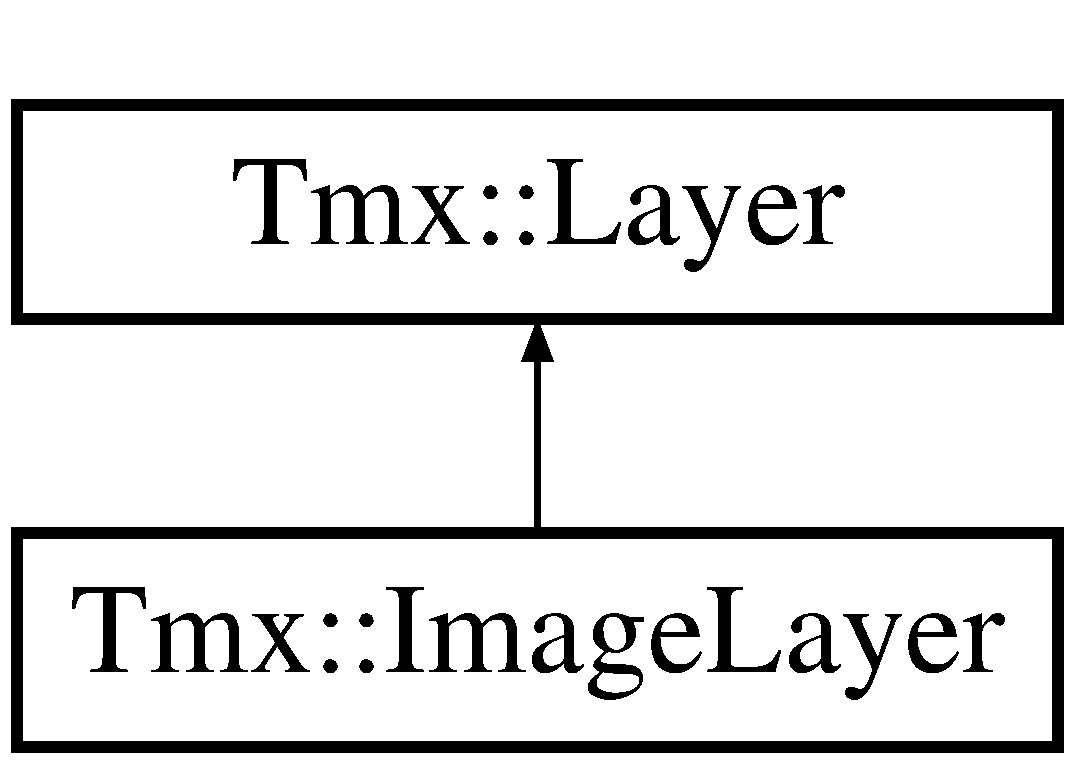
\includegraphics[height=2.000000cm]{classTmx_1_1ImageLayer}
\end{center}
\end{figure}
\subsection*{Public Member Functions}
\begin{DoxyCompactItemize}
\item 
\hypertarget{classTmx_1_1ImageLayer_adac463694d851f0468723318ad511264}{\hyperlink{classTmx_1_1ImageLayer_adac463694d851f0468723318ad511264}{Image\-Layer} (const \hyperlink{classTmx_1_1Map}{Tmx\-::\-Map} $\ast$\-\_\-map)}\label{classTmx_1_1ImageLayer_adac463694d851f0468723318ad511264}

\begin{DoxyCompactList}\small\item\em Construct an \hyperlink{classTmx_1_1ImageLayer}{Image\-Layer} on the given map. \end{DoxyCompactList}\item 
\hypertarget{classTmx_1_1ImageLayer_a5441c6a1393d0b9bea4356f048f8a5c8}{void \hyperlink{classTmx_1_1ImageLayer_a5441c6a1393d0b9bea4356f048f8a5c8}{Parse} (const tinyxml2\-::\-X\-M\-L\-Node $\ast$image\-Layer\-Node)}\label{classTmx_1_1ImageLayer_a5441c6a1393d0b9bea4356f048f8a5c8}

\begin{DoxyCompactList}\small\item\em Parse a \hyperlink{classTmx_1_1ImageLayer}{Image\-Layer} element. \end{DoxyCompactList}\item 
const \hyperlink{classTmx_1_1Image}{Tmx\-::\-Image} $\ast$ \hyperlink{classTmx_1_1ImageLayer_a9963adeceff59ea92933755f13ce8fa9}{Get\-Image} () const 
\begin{DoxyCompactList}\small\item\em Returns a variable containing information about the image of the \hyperlink{classTmx_1_1ImageLayer}{Image\-Layer}. \end{DoxyCompactList}\end{DoxyCompactItemize}


\subsection{Detailed Description}
A class used for holding information about a background image. 

This class has a property set. 

\subsection{Member Function Documentation}
\hypertarget{classTmx_1_1ImageLayer_a9963adeceff59ea92933755f13ce8fa9}{\index{Tmx\-::\-Image\-Layer@{Tmx\-::\-Image\-Layer}!Get\-Image@{Get\-Image}}
\index{Get\-Image@{Get\-Image}!Tmx::ImageLayer@{Tmx\-::\-Image\-Layer}}
\subsubsection[{Get\-Image}]{\setlength{\rightskip}{0pt plus 5cm}const {\bf Tmx\-::\-Image}$\ast$ Tmx\-::\-Image\-Layer\-::\-Get\-Image (
\begin{DoxyParamCaption}
{}
\end{DoxyParamCaption}
) const\hspace{0.3cm}{\ttfamily [inline]}}}\label{classTmx_1_1ImageLayer_a9963adeceff59ea92933755f13ce8fa9}


Returns a variable containing information about the image of the \hyperlink{classTmx_1_1ImageLayer}{Image\-Layer}. 



The documentation for this class was generated from the following files\-:\begin{DoxyCompactItemize}
\item 
/home/travis/build/sainteos/tmxparser/src/Tmx\-Image\-Layer.\-h\item 
/home/travis/build/sainteos/tmxparser/src/Tmx\-Image\-Layer.\-cpp\end{DoxyCompactItemize}

\hypertarget{classTmx_1_1Layer}{\section{Tmx\-:\-:Layer Class Reference}
\label{classTmx_1_1Layer}\index{Tmx\-::\-Layer@{Tmx\-::\-Layer}}
}


Base class for other layer types.  




{\ttfamily \#include $<$Tmx\-Layer.\-h$>$}

Inheritance diagram for Tmx\-:\-:Layer\-:\begin{figure}[H]
\begin{center}
\leavevmode
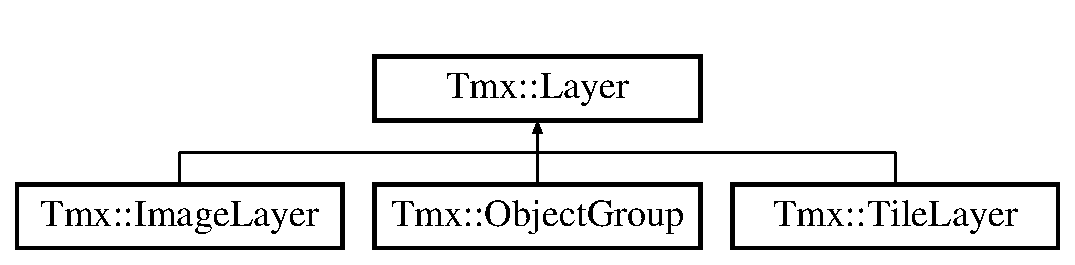
\includegraphics[height=2.000000cm]{classTmx_1_1Layer}
\end{center}
\end{figure}
\subsection*{Public Member Functions}
\begin{DoxyCompactItemize}
\item 
\hypertarget{classTmx_1_1Layer_a6984126fbda7aecb74f4a124740e8672}{\hyperlink{classTmx_1_1Layer_a6984126fbda7aecb74f4a124740e8672}{Layer} (const \hyperlink{classTmx_1_1Map}{Tmx\-::\-Map} $\ast$\-\_\-map, const std\-::string \-\_\-name, const int \-\_\-x, const int \-\_\-y, const int \-\_\-width, const int \-\_\-height, const float \-\_\-opacity, const bool \-\_\-visible, const Layer\-Type \-\_\-layer\-Type)}\label{classTmx_1_1Layer_a6984126fbda7aecb74f4a124740e8672}

\begin{DoxyCompactList}\small\item\em Construct a new \hyperlink{classTmx_1_1Layer}{Layer}. \end{DoxyCompactList}\item 
\hypertarget{classTmx_1_1Layer_adbc29ca32a7d2172f47787d93187401c}{virtual void \hyperlink{classTmx_1_1Layer_adbc29ca32a7d2172f47787d93187401c}{Parse} (const tinyxml2\-::\-X\-M\-L\-Node $\ast$layer\-Node)=0}\label{classTmx_1_1Layer_adbc29ca32a7d2172f47787d93187401c}

\begin{DoxyCompactList}\small\item\em Parse a layer element. \end{DoxyCompactList}\item 
\hypertarget{classTmx_1_1Layer_a88f85f9315074c6c57fedc9352ac326c}{const \hyperlink{classTmx_1_1Map}{Tmx\-::\-Map} $\ast$ \hyperlink{classTmx_1_1Layer_a88f85f9315074c6c57fedc9352ac326c}{map\-Get\-Map} () const }\label{classTmx_1_1Layer_a88f85f9315074c6c57fedc9352ac326c}

\begin{DoxyCompactList}\small\item\em Get the pointer to the parent map. \end{DoxyCompactList}\item 
\hypertarget{classTmx_1_1Layer_a3896ff18af7bf93d73f7a42cf7c34f14}{const std\-::string \& \hyperlink{classTmx_1_1Layer_a3896ff18af7bf93d73f7a42cf7c34f14}{Get\-Name} () const }\label{classTmx_1_1Layer_a3896ff18af7bf93d73f7a42cf7c34f14}

\begin{DoxyCompactList}\small\item\em Get the name of the layer. \end{DoxyCompactList}\item 
\hypertarget{classTmx_1_1Layer_afc3899eaffe2425ad31ea3035a34c2ca}{int \hyperlink{classTmx_1_1Layer_afc3899eaffe2425ad31ea3035a34c2ca}{Get\-X} () const }\label{classTmx_1_1Layer_afc3899eaffe2425ad31ea3035a34c2ca}

\begin{DoxyCompactList}\small\item\em Get the value of the x attribute of the layer. Means different things for different layer types. \end{DoxyCompactList}\item 
\hypertarget{classTmx_1_1Layer_aa65a3ed0d53c60ab0356e256b3553c3d}{int \hyperlink{classTmx_1_1Layer_aa65a3ed0d53c60ab0356e256b3553c3d}{Get\-Y} () const }\label{classTmx_1_1Layer_aa65a3ed0d53c60ab0356e256b3553c3d}

\begin{DoxyCompactList}\small\item\em Get the value of the y attribute of the layer. Means different things for different layer types. \end{DoxyCompactList}\item 
\hypertarget{classTmx_1_1Layer_a199a01de350b86975e9473a9aa491de4}{int \hyperlink{classTmx_1_1Layer_a199a01de350b86975e9473a9aa491de4}{Get\-Width} () const }\label{classTmx_1_1Layer_a199a01de350b86975e9473a9aa491de4}

\begin{DoxyCompactList}\small\item\em Get the width of the layer, in tiles. Only used in tile layers. \end{DoxyCompactList}\item 
\hypertarget{classTmx_1_1Layer_a6f8cf75b8249eb4c1e62256cde828183}{int \hyperlink{classTmx_1_1Layer_a6f8cf75b8249eb4c1e62256cde828183}{Get\-Height} () const }\label{classTmx_1_1Layer_a6f8cf75b8249eb4c1e62256cde828183}

\begin{DoxyCompactList}\small\item\em Get the height of the layer, in tiles. Only used in tile layers. \end{DoxyCompactList}\item 
\hypertarget{classTmx_1_1Layer_a093f75d1b7e5afbdf4ce3c3efcdc8182}{float \hyperlink{classTmx_1_1Layer_a093f75d1b7e5afbdf4ce3c3efcdc8182}{Get\-Opacity} () const }\label{classTmx_1_1Layer_a093f75d1b7e5afbdf4ce3c3efcdc8182}

\begin{DoxyCompactList}\small\item\em Get the opacity of the layer. \end{DoxyCompactList}\item 
\hypertarget{classTmx_1_1Layer_a231832ce15394aa1c6b1a61db561a8dd}{bool \hyperlink{classTmx_1_1Layer_a231832ce15394aa1c6b1a61db561a8dd}{Is\-Visible} () const }\label{classTmx_1_1Layer_a231832ce15394aa1c6b1a61db561a8dd}

\begin{DoxyCompactList}\small\item\em Get the visibility of the layer. \end{DoxyCompactList}\item 
\hypertarget{classTmx_1_1Layer_ac404e49efb50d98afcb468283dc20640}{const \hyperlink{classTmx_1_1PropertySet}{Tmx\-::\-Property\-Set} \& \hyperlink{classTmx_1_1Layer_ac404e49efb50d98afcb468283dc20640}{Get\-Properties} () const }\label{classTmx_1_1Layer_ac404e49efb50d98afcb468283dc20640}

\begin{DoxyCompactList}\small\item\em Get the property set. \end{DoxyCompactList}\item 
\hypertarget{classTmx_1_1Layer_a6d77cf7f59bf82be8c97d7d6ab26bfae}{int \hyperlink{classTmx_1_1Layer_a6d77cf7f59bf82be8c97d7d6ab26bfae}{Get\-Z\-Order} () const }\label{classTmx_1_1Layer_a6d77cf7f59bf82be8c97d7d6ab26bfae}

\begin{DoxyCompactList}\small\item\em Get the zorder of the layer. \end{DoxyCompactList}\item 
\hypertarget{classTmx_1_1Layer_ac467e3cb03d7e9a1d8199d4b33f5a78b}{void \hyperlink{classTmx_1_1Layer_ac467e3cb03d7e9a1d8199d4b33f5a78b}{Set\-Z\-Order} (int z)}\label{classTmx_1_1Layer_ac467e3cb03d7e9a1d8199d4b33f5a78b}

\begin{DoxyCompactList}\small\item\em Set the zorder of the layer. \end{DoxyCompactList}\item 
\hypertarget{classTmx_1_1Layer_a27687188f81c797c3a3c8a62bf7282ff}{int \hyperlink{classTmx_1_1Layer_a27687188f81c797c3a3c8a62bf7282ff}{Get\-Parse\-Order} () const }\label{classTmx_1_1Layer_a27687188f81c797c3a3c8a62bf7282ff}

\begin{DoxyCompactList}\small\item\em Get the parse order of the layer. \end{DoxyCompactList}\item 
\hypertarget{classTmx_1_1Layer_ab34f5b1a9ad759005b5bdb88974b233f}{Tmx\-::\-Layer\-Type \hyperlink{classTmx_1_1Layer_ab34f5b1a9ad759005b5bdb88974b233f}{Get\-Layer\-Type} () const }\label{classTmx_1_1Layer_ab34f5b1a9ad759005b5bdb88974b233f}

\begin{DoxyCompactList}\small\item\em Get the type of the layer. \end{DoxyCompactList}\end{DoxyCompactItemize}


\subsection{Detailed Description}
Base class for other layer types. 

The documentation for this class was generated from the following files\-:\begin{DoxyCompactItemize}
\item 
/home/travis/build/sainteos/tmxparser/src/Tmx\-Layer.\-h\item 
/home/travis/build/sainteos/tmxparser/src/Tmx\-Layer.\-cpp\end{DoxyCompactItemize}

\hypertarget{classTmx_1_1Map}{\section{Tmx\-:\-:Map Class Reference}
\label{classTmx_1_1Map}\index{Tmx\-::\-Map@{Tmx\-::\-Map}}
}


This class is the root class of the parser.  




{\ttfamily \#include $<$Tmx\-Map.\-h$>$}

\subsection*{Public Member Functions}
\begin{DoxyCompactItemize}
\item 
void \hyperlink{classTmx_1_1Map_a6402c3b55e687cd561b3eb3c16341d64}{Parse\-File} (const std\-::string \&file\-Name)
\begin{DoxyCompactList}\small\item\em Read a file and parse it. \end{DoxyCompactList}\item 
\hypertarget{classTmx_1_1Map_a5b1e7fb80a243bf439eb59143588e6f1}{void \hyperlink{classTmx_1_1Map_a5b1e7fb80a243bf439eb59143588e6f1}{Parse\-Text} (const std\-::string \&text)}\label{classTmx_1_1Map_a5b1e7fb80a243bf439eb59143588e6f1}

\begin{DoxyCompactList}\small\item\em Parse text containing T\-M\-X formatted X\-M\-L. \end{DoxyCompactList}\item 
\hypertarget{classTmx_1_1Map_ac8d4b67bc03893c8ddf94e5ca84addd5}{const std\-::string \& \hyperlink{classTmx_1_1Map_ac8d4b67bc03893c8ddf94e5ca84addd5}{Get\-Filename} () const }\label{classTmx_1_1Map_ac8d4b67bc03893c8ddf94e5ca84addd5}

\begin{DoxyCompactList}\small\item\em Get the filename used to read the map. \end{DoxyCompactList}\item 
\hypertarget{classTmx_1_1Map_a26f2a6a44512f00404bf800f31fc4b90}{const std\-::string \& \hyperlink{classTmx_1_1Map_a26f2a6a44512f00404bf800f31fc4b90}{Get\-Filepath} () const }\label{classTmx_1_1Map_a26f2a6a44512f00404bf800f31fc4b90}

\begin{DoxyCompactList}\small\item\em Get a path to the directory of the map file if any. \end{DoxyCompactList}\item 
\hypertarget{classTmx_1_1Map_a26f1b6f42e6fba38764d8a670bbc9634}{\hyperlink{classTmx_1_1Color}{Tmx\-::\-Color} \hyperlink{classTmx_1_1Map_a26f1b6f42e6fba38764d8a670bbc9634}{Get\-Background\-Color} () const }\label{classTmx_1_1Map_a26f1b6f42e6fba38764d8a670bbc9634}

\begin{DoxyCompactList}\small\item\em Get the background color of the map file. If unset, return a fully transparent color. \end{DoxyCompactList}\item 
\hypertarget{classTmx_1_1Map_a0293a108d6dad2581b7db37adeee1474}{double \hyperlink{classTmx_1_1Map_a0293a108d6dad2581b7db37adeee1474}{Get\-Version} () const }\label{classTmx_1_1Map_a0293a108d6dad2581b7db37adeee1474}

\begin{DoxyCompactList}\small\item\em Get the version of the map. \end{DoxyCompactList}\item 
\hypertarget{classTmx_1_1Map_a7cc9f5a5d57b0d118d12f759e1b479b6}{Tmx\-::\-Map\-Orientation \hyperlink{classTmx_1_1Map_a7cc9f5a5d57b0d118d12f759e1b479b6}{Get\-Orientation} () const }\label{classTmx_1_1Map_a7cc9f5a5d57b0d118d12f759e1b479b6}

\begin{DoxyCompactList}\small\item\em Get the orientation of the map. \end{DoxyCompactList}\item 
\hypertarget{classTmx_1_1Map_aafe9c6f1b5ed6649145875f4c525b2bf}{Tmx\-::\-Map\-Render\-Order \hyperlink{classTmx_1_1Map_aafe9c6f1b5ed6649145875f4c525b2bf}{Get\-Render\-Order} () const }\label{classTmx_1_1Map_aafe9c6f1b5ed6649145875f4c525b2bf}

\begin{DoxyCompactList}\small\item\em Get the render order of the map. \end{DoxyCompactList}\item 
\hypertarget{classTmx_1_1Map_a442d8d11d30de6c5f72e300636969766}{Tmx\-::\-Map\-Stagger\-Axis \hyperlink{classTmx_1_1Map_a442d8d11d30de6c5f72e300636969766}{Get\-Stagger\-Axis} () const }\label{classTmx_1_1Map_a442d8d11d30de6c5f72e300636969766}

\begin{DoxyCompactList}\small\item\em Get the stagger axis of the map. \end{DoxyCompactList}\item 
\hypertarget{classTmx_1_1Map_a6fce5949f2c6c42764f1eb2dbdee8007}{Tmx\-::\-Map\-Stagger\-Index \hyperlink{classTmx_1_1Map_a6fce5949f2c6c42764f1eb2dbdee8007}{Get\-Stagger\-Index} () const }\label{classTmx_1_1Map_a6fce5949f2c6c42764f1eb2dbdee8007}

\begin{DoxyCompactList}\small\item\em Get the stagger index of the map. \end{DoxyCompactList}\item 
\hypertarget{classTmx_1_1Map_a725e44f4122460bd8aafecc1849a2163}{int \hyperlink{classTmx_1_1Map_a725e44f4122460bd8aafecc1849a2163}{Get\-Width} () const }\label{classTmx_1_1Map_a725e44f4122460bd8aafecc1849a2163}

\begin{DoxyCompactList}\small\item\em Get the width of the map, in tiles. \end{DoxyCompactList}\item 
\hypertarget{classTmx_1_1Map_ad092fdee9e291e9bbc848e811b321981}{int \hyperlink{classTmx_1_1Map_ad092fdee9e291e9bbc848e811b321981}{Get\-Height} () const }\label{classTmx_1_1Map_ad092fdee9e291e9bbc848e811b321981}

\begin{DoxyCompactList}\small\item\em Get the height of the map, in tiles. \end{DoxyCompactList}\item 
\hypertarget{classTmx_1_1Map_acc625a29299129b6f1d534bb768c0e3f}{int \hyperlink{classTmx_1_1Map_acc625a29299129b6f1d534bb768c0e3f}{Get\-Tile\-Width} () const }\label{classTmx_1_1Map_acc625a29299129b6f1d534bb768c0e3f}

\begin{DoxyCompactList}\small\item\em Get the width of a tile, in pixels. \end{DoxyCompactList}\item 
\hypertarget{classTmx_1_1Map_a43bdd29747a818d528f248edc2fbb433}{int \hyperlink{classTmx_1_1Map_a43bdd29747a818d528f248edc2fbb433}{Get\-Tile\-Height} () const }\label{classTmx_1_1Map_a43bdd29747a818d528f248edc2fbb433}

\begin{DoxyCompactList}\small\item\em Get the height of a tile, in pixels. \end{DoxyCompactList}\item 
\hypertarget{classTmx_1_1Map_ae7f78454e34aad16e21638899b7731cb}{int \hyperlink{classTmx_1_1Map_ae7f78454e34aad16e21638899b7731cb}{Get\-Next\-Object\-Id} () const }\label{classTmx_1_1Map_ae7f78454e34aad16e21638899b7731cb}

\begin{DoxyCompactList}\small\item\em Get the next object id. \end{DoxyCompactList}\item 
\hypertarget{classTmx_1_1Map_a33869535415f6f78cbd7d723ce22caf1}{int \hyperlink{classTmx_1_1Map_a33869535415f6f78cbd7d723ce22caf1}{Get\-Hexside\-Length} () const }\label{classTmx_1_1Map_a33869535415f6f78cbd7d723ce22caf1}

\begin{DoxyCompactList}\small\item\em Get the hexside length. \end{DoxyCompactList}\item 
\hypertarget{classTmx_1_1Map_aea9eb94cf709bd31f0cb4cc033f1c96c}{const \hyperlink{classTmx_1_1Layer}{Tmx\-::\-Layer} $\ast$ \hyperlink{classTmx_1_1Map_aea9eb94cf709bd31f0cb4cc033f1c96c}{Get\-Layer} (int index) const }\label{classTmx_1_1Map_aea9eb94cf709bd31f0cb4cc033f1c96c}

\begin{DoxyCompactList}\small\item\em Get the layer at a certain index. \end{DoxyCompactList}\item 
\hypertarget{classTmx_1_1Map_ad2a948b09fd47d4370830498ace72cb6}{int \hyperlink{classTmx_1_1Map_ad2a948b09fd47d4370830498ace72cb6}{Get\-Num\-Layers} () const }\label{classTmx_1_1Map_ad2a948b09fd47d4370830498ace72cb6}

\begin{DoxyCompactList}\small\item\em Get the amount of layers. \end{DoxyCompactList}\item 
\hypertarget{classTmx_1_1Map_a60def10fd94a3027d70e80876c836286}{const std\-::vector$<$ \hyperlink{classTmx_1_1Layer}{Tmx\-::\-Layer} $\ast$ $>$ \& \hyperlink{classTmx_1_1Map_a60def10fd94a3027d70e80876c836286}{Get\-Layers} () const }\label{classTmx_1_1Map_a60def10fd94a3027d70e80876c836286}

\begin{DoxyCompactList}\small\item\em Get the whole layers collection. \end{DoxyCompactList}\item 
\hypertarget{classTmx_1_1Map_a20af7306c305815dad3023c8bd06bb15}{const \hyperlink{classTmx_1_1TileLayer}{Tmx\-::\-Tile\-Layer} $\ast$ \hyperlink{classTmx_1_1Map_a20af7306c305815dad3023c8bd06bb15}{Get\-Tile\-Layer} (int index) const }\label{classTmx_1_1Map_a20af7306c305815dad3023c8bd06bb15}

\begin{DoxyCompactList}\small\item\em Get the tile layer at a certain index. \end{DoxyCompactList}\item 
\hypertarget{classTmx_1_1Map_abe0294845cf427b2446b36fec48ebd77}{int \hyperlink{classTmx_1_1Map_abe0294845cf427b2446b36fec48ebd77}{Get\-Num\-Tile\-Layers} () const }\label{classTmx_1_1Map_abe0294845cf427b2446b36fec48ebd77}

\begin{DoxyCompactList}\small\item\em Get the amount of tile layers. \end{DoxyCompactList}\item 
\hypertarget{classTmx_1_1Map_a1e6a0eb80d60ef16af3ccc438ab8716f}{const std\-::vector\\*
$<$ \hyperlink{classTmx_1_1TileLayer}{Tmx\-::\-Tile\-Layer} $\ast$ $>$ \& \hyperlink{classTmx_1_1Map_a1e6a0eb80d60ef16af3ccc438ab8716f}{Get\-Tile\-Layers} () const }\label{classTmx_1_1Map_a1e6a0eb80d60ef16af3ccc438ab8716f}

\begin{DoxyCompactList}\small\item\em Get the whole collection of tile layers. \end{DoxyCompactList}\item 
\hypertarget{classTmx_1_1Map_a46c05a71369d22cfa55367b07d771b11}{const \hyperlink{classTmx_1_1ObjectGroup}{Tmx\-::\-Object\-Group} $\ast$ \hyperlink{classTmx_1_1Map_a46c05a71369d22cfa55367b07d771b11}{Get\-Object\-Group} (int index) const }\label{classTmx_1_1Map_a46c05a71369d22cfa55367b07d771b11}

\begin{DoxyCompactList}\small\item\em Get the object group at a certain index. \end{DoxyCompactList}\item 
\hypertarget{classTmx_1_1Map_aae09a01218a3fe3540347fb2ed65fccd}{int \hyperlink{classTmx_1_1Map_aae09a01218a3fe3540347fb2ed65fccd}{Get\-Num\-Object\-Groups} () const }\label{classTmx_1_1Map_aae09a01218a3fe3540347fb2ed65fccd}

\begin{DoxyCompactList}\small\item\em Get the amount of object groups. \end{DoxyCompactList}\item 
\hypertarget{classTmx_1_1Map_adcd29ef72e9649bd05a3579e9c61ed68}{const std\-::vector\\*
$<$ \hyperlink{classTmx_1_1ObjectGroup}{Tmx\-::\-Object\-Group} $\ast$ $>$ \& \hyperlink{classTmx_1_1Map_adcd29ef72e9649bd05a3579e9c61ed68}{Get\-Object\-Groups} () const }\label{classTmx_1_1Map_adcd29ef72e9649bd05a3579e9c61ed68}

\begin{DoxyCompactList}\small\item\em Get the whole collection of object groups. \end{DoxyCompactList}\item 
\hypertarget{classTmx_1_1Map_ad9c7fcc05963002e5c7efa71f4ba0cdb}{const \hyperlink{classTmx_1_1ImageLayer}{Tmx\-::\-Image\-Layer} $\ast$ \hyperlink{classTmx_1_1Map_ad9c7fcc05963002e5c7efa71f4ba0cdb}{Get\-Image\-Layer} (int index) const }\label{classTmx_1_1Map_ad9c7fcc05963002e5c7efa71f4ba0cdb}

\begin{DoxyCompactList}\small\item\em Get the image layer at a certain index. \end{DoxyCompactList}\item 
\hypertarget{classTmx_1_1Map_a3b671ac157c5ff008e031896162dd90b}{int \hyperlink{classTmx_1_1Map_a3b671ac157c5ff008e031896162dd90b}{Get\-Num\-Image\-Layers} () const }\label{classTmx_1_1Map_a3b671ac157c5ff008e031896162dd90b}

\begin{DoxyCompactList}\small\item\em Get the amount of image layers. \end{DoxyCompactList}\item 
\hypertarget{classTmx_1_1Map_a6139d52f06e655609f9b444c681dc82e}{const std\-::vector\\*
$<$ \hyperlink{classTmx_1_1ImageLayer}{Tmx\-::\-Image\-Layer} $\ast$ $>$ \& \hyperlink{classTmx_1_1Map_a6139d52f06e655609f9b444c681dc82e}{Get\-Image\-Layers} () const }\label{classTmx_1_1Map_a6139d52f06e655609f9b444c681dc82e}

\begin{DoxyCompactList}\small\item\em Get the whole collection of image layers. \end{DoxyCompactList}\item 
\hypertarget{classTmx_1_1Map_ae4eaf84225934c655b58dd8777affa57}{int \hyperlink{classTmx_1_1Map_ae4eaf84225934c655b58dd8777affa57}{Find\-Tileset\-Index} (int gid) const }\label{classTmx_1_1Map_ae4eaf84225934c655b58dd8777affa57}

\begin{DoxyCompactList}\small\item\em Find the tileset index for a tileset using a tile gid. \end{DoxyCompactList}\item 
\hypertarget{classTmx_1_1Map_ad6fc54dec9788c9e5875366cfcce7e75}{const \hyperlink{classTmx_1_1Tileset}{Tmx\-::\-Tileset} $\ast$ \hyperlink{classTmx_1_1Map_ad6fc54dec9788c9e5875366cfcce7e75}{Find\-Tileset} (int gid) const }\label{classTmx_1_1Map_ad6fc54dec9788c9e5875366cfcce7e75}

\begin{DoxyCompactList}\small\item\em Find a tileset for a specific gid. \end{DoxyCompactList}\item 
\hypertarget{classTmx_1_1Map_aa2a15a2928afd35d6bdb679e8cf9c1c5}{const \hyperlink{classTmx_1_1Tileset}{Tmx\-::\-Tileset} $\ast$ \hyperlink{classTmx_1_1Map_aa2a15a2928afd35d6bdb679e8cf9c1c5}{Get\-Tileset} (int index) const }\label{classTmx_1_1Map_aa2a15a2928afd35d6bdb679e8cf9c1c5}

\begin{DoxyCompactList}\small\item\em Get a tileset by an index. \end{DoxyCompactList}\item 
\hypertarget{classTmx_1_1Map_ace78d988082829b6ddbd14f9cb7b848b}{int \hyperlink{classTmx_1_1Map_ace78d988082829b6ddbd14f9cb7b848b}{Get\-Num\-Tilesets} () const }\label{classTmx_1_1Map_ace78d988082829b6ddbd14f9cb7b848b}

\begin{DoxyCompactList}\small\item\em Get the amount of tilesets. \end{DoxyCompactList}\item 
\hypertarget{classTmx_1_1Map_a04a2b25c901724a24d24ff27e205533d}{const std\-::vector\\*
$<$ \hyperlink{classTmx_1_1Tileset}{Tmx\-::\-Tileset} $\ast$ $>$ \& \hyperlink{classTmx_1_1Map_a04a2b25c901724a24d24ff27e205533d}{Get\-Tilesets} () const }\label{classTmx_1_1Map_a04a2b25c901724a24d24ff27e205533d}

\begin{DoxyCompactList}\small\item\em Get the collection of tilesets. \end{DoxyCompactList}\item 
\hypertarget{classTmx_1_1Map_af6e7c1d916c6da7b407df74a0ff49d99}{bool \hyperlink{classTmx_1_1Map_af6e7c1d916c6da7b407df74a0ff49d99}{Has\-Error} () const }\label{classTmx_1_1Map_af6e7c1d916c6da7b407df74a0ff49d99}

\begin{DoxyCompactList}\small\item\em Get whether there was an error or not. \end{DoxyCompactList}\item 
\hypertarget{classTmx_1_1Map_a88ea91dee43fedf004b5a284feda1299}{const std\-::string \& \hyperlink{classTmx_1_1Map_a88ea91dee43fedf004b5a284feda1299}{Get\-Error\-Text} () const }\label{classTmx_1_1Map_a88ea91dee43fedf004b5a284feda1299}

\begin{DoxyCompactList}\small\item\em Get an error string containing the error in text format. \end{DoxyCompactList}\item 
\hypertarget{classTmx_1_1Map_a67421419f5b9ffb2d260dbcd89fd42b5}{unsigned char \hyperlink{classTmx_1_1Map_a67421419f5b9ffb2d260dbcd89fd42b5}{Get\-Error\-Code} () const }\label{classTmx_1_1Map_a67421419f5b9ffb2d260dbcd89fd42b5}

\begin{DoxyCompactList}\small\item\em Get a number that identifies the error. (T\-M\-X\-\_\- preceded constants) \end{DoxyCompactList}\item 
\hypertarget{classTmx_1_1Map_a3e784f25f099709e12ab951abeb6d511}{const \hyperlink{classTmx_1_1PropertySet}{Tmx\-::\-Property\-Set} \& \hyperlink{classTmx_1_1Map_a3e784f25f099709e12ab951abeb6d511}{Get\-Properties} () const }\label{classTmx_1_1Map_a3e784f25f099709e12ab951abeb6d511}

\begin{DoxyCompactList}\small\item\em Get the property set. \end{DoxyCompactList}\end{DoxyCompactItemize}


\subsection{Detailed Description}
This class is the root class of the parser. 

It has all of the information in regard to the T\-M\-X file. This class has a property set. 

\subsection{Member Function Documentation}
\hypertarget{classTmx_1_1Map_a6402c3b55e687cd561b3eb3c16341d64}{\index{Tmx\-::\-Map@{Tmx\-::\-Map}!Parse\-File@{Parse\-File}}
\index{Parse\-File@{Parse\-File}!Tmx::Map@{Tmx\-::\-Map}}
\subsubsection[{Parse\-File}]{\setlength{\rightskip}{0pt plus 5cm}void Tmx\-::\-Map\-::\-Parse\-File (
\begin{DoxyParamCaption}
\item[{const std\-::string \&}]{file\-Name}
\end{DoxyParamCaption}
)}}\label{classTmx_1_1Map_a6402c3b55e687cd561b3eb3c16341d64}


Read a file and parse it. 

Note\-: use '/' instead of '\textbackslash{}' as it is using '/' to find the path. 

The documentation for this class was generated from the following files\-:\begin{DoxyCompactItemize}
\item 
/home/travis/build/sainteos/tmxparser/src/Tmx\-Map.\-h\item 
/home/travis/build/sainteos/tmxparser/src/Tmx\-Map.\-cpp\end{DoxyCompactItemize}

\hypertarget{structTmx_1_1MapTile}{\section{Tmx\-:\-:Map\-Tile Struct Reference}
\label{structTmx_1_1MapTile}\index{Tmx\-::\-Map\-Tile@{Tmx\-::\-Map\-Tile}}
}


Struct to store information about a specific tile in the map layer.  




{\ttfamily \#include $<$Tmx\-Map\-Tile.\-h$>$}

\subsection*{Public Member Functions}
\begin{DoxyCompactItemize}
\item 
\hypertarget{structTmx_1_1MapTile_a1e914d4cb599e79ade3cf178879b9135}{\hyperlink{structTmx_1_1MapTile_a1e914d4cb599e79ade3cf178879b9135}{Map\-Tile} ()}\label{structTmx_1_1MapTile_a1e914d4cb599e79ade3cf178879b9135}

\begin{DoxyCompactList}\small\item\em Default constructor. \end{DoxyCompactList}\item 
\hyperlink{structTmx_1_1MapTile_a2ce4eaefeb86a127535521c32eed9cf3}{Map\-Tile} (unsigned \-\_\-gid, int \-\_\-tileset\-First\-Gid, unsigned \-\_\-tileset\-Id)
\begin{DoxyCompactList}\small\item\em Will take a gid and read the attributes from the first two bits of it. \end{DoxyCompactList}\end{DoxyCompactItemize}
\subsection*{Public Attributes}
\begin{DoxyCompactItemize}
\item 
\hypertarget{structTmx_1_1MapTile_a1229850428649e3bbb961c6e48907de5}{int \hyperlink{structTmx_1_1MapTile_a1229850428649e3bbb961c6e48907de5}{tileset\-Id}}\label{structTmx_1_1MapTile_a1229850428649e3bbb961c6e48907de5}

\begin{DoxyCompactList}\small\item\em \hyperlink{classTmx_1_1Tileset}{Tileset} id. \end{DoxyCompactList}\item 
\hypertarget{structTmx_1_1MapTile_a5e5e67a6ef3d7908885bce9d522e3d51}{unsigned \hyperlink{structTmx_1_1MapTile_a5e5e67a6ef3d7908885bce9d522e3d51}{id}}\label{structTmx_1_1MapTile_a5e5e67a6ef3d7908885bce9d522e3d51}

\begin{DoxyCompactList}\small\item\em Id. \end{DoxyCompactList}\item 
\hypertarget{structTmx_1_1MapTile_ae942fff5e6cb0f7fd9305ea419c156cd}{unsigned \hyperlink{structTmx_1_1MapTile_ae942fff5e6cb0f7fd9305ea419c156cd}{gid}}\label{structTmx_1_1MapTile_ae942fff5e6cb0f7fd9305ea419c156cd}

\begin{DoxyCompactList}\small\item\em Gid. \end{DoxyCompactList}\item 
\hypertarget{structTmx_1_1MapTile_ae64471c7caba072e91be5cbecd0afd3d}{bool \hyperlink{structTmx_1_1MapTile_ae64471c7caba072e91be5cbecd0afd3d}{flipped\-Horizontally}}\label{structTmx_1_1MapTile_ae64471c7caba072e91be5cbecd0afd3d}

\begin{DoxyCompactList}\small\item\em True when the tile should be drawn flipped horizontally. \end{DoxyCompactList}\item 
\hypertarget{structTmx_1_1MapTile_a86f732bd548caf59ac25755663871fbe}{bool \hyperlink{structTmx_1_1MapTile_a86f732bd548caf59ac25755663871fbe}{flipped\-Vertically}}\label{structTmx_1_1MapTile_a86f732bd548caf59ac25755663871fbe}

\begin{DoxyCompactList}\small\item\em True when the tile should be drawn flipped vertically. \end{DoxyCompactList}\item 
\hypertarget{structTmx_1_1MapTile_a4ed16706d5ed2adab6f03a1324deb751}{bool \hyperlink{structTmx_1_1MapTile_a4ed16706d5ed2adab6f03a1324deb751}{flipped\-Diagonally}}\label{structTmx_1_1MapTile_a4ed16706d5ed2adab6f03a1324deb751}

\begin{DoxyCompactList}\small\item\em True when the tile should be drawn flipped diagonally. \end{DoxyCompactList}\end{DoxyCompactItemize}


\subsection{Detailed Description}
Struct to store information about a specific tile in the map layer. 

\subsection{Constructor \& Destructor Documentation}
\hypertarget{structTmx_1_1MapTile_a2ce4eaefeb86a127535521c32eed9cf3}{\index{Tmx\-::\-Map\-Tile@{Tmx\-::\-Map\-Tile}!Map\-Tile@{Map\-Tile}}
\index{Map\-Tile@{Map\-Tile}!Tmx::MapTile@{Tmx\-::\-Map\-Tile}}
\subsubsection[{Map\-Tile}]{\setlength{\rightskip}{0pt plus 5cm}Tmx\-::\-Map\-Tile\-::\-Map\-Tile (
\begin{DoxyParamCaption}
\item[{unsigned}]{\-\_\-gid, }
\item[{int}]{\-\_\-tileset\-First\-Gid, }
\item[{unsigned}]{\-\_\-tileset\-Id}
\end{DoxyParamCaption}
)\hspace{0.3cm}{\ttfamily [inline]}}}\label{structTmx_1_1MapTile_a2ce4eaefeb86a127535521c32eed9cf3}


Will take a gid and read the attributes from the first two bits of it. 



The documentation for this struct was generated from the following file\-:\begin{DoxyCompactItemize}
\item 
/home/travis/build/sainteos/tmxparser/src/Tmx\-Map\-Tile.\-h\end{DoxyCompactItemize}

\hypertarget{classTmx_1_1Object}{\section{Tmx\-:\-:Object Class Reference}
\label{classTmx_1_1Object}\index{Tmx\-::\-Object@{Tmx\-::\-Object}}
}


Class used for representing a single object from the objectgroup.  




{\ttfamily \#include $<$Tmx\-Object.\-h$>$}

\subsection*{Public Member Functions}
\begin{DoxyCompactItemize}
\item 
\hypertarget{classTmx_1_1Object_a7065e21be60a3534997bc89648407d48}{void \hyperlink{classTmx_1_1Object_a7065e21be60a3534997bc89648407d48}{Parse} (const tinyxml2\-::\-X\-M\-L\-Node $\ast$object\-Node)}\label{classTmx_1_1Object_a7065e21be60a3534997bc89648407d48}

\begin{DoxyCompactList}\small\item\em Parse an object node. \end{DoxyCompactList}\item 
\hypertarget{classTmx_1_1Object_ada7d925bd462b3b8b7ddedf0e8891a3d}{const std\-::string \& \hyperlink{classTmx_1_1Object_ada7d925bd462b3b8b7ddedf0e8891a3d}{Get\-Name} () const }\label{classTmx_1_1Object_ada7d925bd462b3b8b7ddedf0e8891a3d}

\begin{DoxyCompactList}\small\item\em Get the name of the object. \end{DoxyCompactList}\item 
\hypertarget{classTmx_1_1Object_a99cb9247d2bebbe45c7cccc58cf47737}{const std\-::string \& \hyperlink{classTmx_1_1Object_a99cb9247d2bebbe45c7cccc58cf47737}{Get\-Type} () const }\label{classTmx_1_1Object_a99cb9247d2bebbe45c7cccc58cf47737}

\begin{DoxyCompactList}\small\item\em Get the type of the object. \end{DoxyCompactList}\item 
\hypertarget{classTmx_1_1Object_a4491f0abc015b7fb1c845bae7dc6008d}{int \hyperlink{classTmx_1_1Object_a4491f0abc015b7fb1c845bae7dc6008d}{Get\-X} () const }\label{classTmx_1_1Object_a4491f0abc015b7fb1c845bae7dc6008d}

\begin{DoxyCompactList}\small\item\em Get the left side of the object, in pixels. \end{DoxyCompactList}\item 
\hypertarget{classTmx_1_1Object_af4417421feb6732d973e2aa0771f9b1e}{int \hyperlink{classTmx_1_1Object_af4417421feb6732d973e2aa0771f9b1e}{Get\-Y} () const }\label{classTmx_1_1Object_af4417421feb6732d973e2aa0771f9b1e}

\begin{DoxyCompactList}\small\item\em Get the top side of the object, in pixels. \end{DoxyCompactList}\item 
\hypertarget{classTmx_1_1Object_a5f34e674147cd764e874e0f59c3427fc}{int \hyperlink{classTmx_1_1Object_a5f34e674147cd764e874e0f59c3427fc}{Get\-Width} () const }\label{classTmx_1_1Object_a5f34e674147cd764e874e0f59c3427fc}

\begin{DoxyCompactList}\small\item\em Get the width of the object, in pixels. \end{DoxyCompactList}\item 
\hypertarget{classTmx_1_1Object_a8f38dc66b0a7c9144282e7dc9c099e40}{int \hyperlink{classTmx_1_1Object_a8f38dc66b0a7c9144282e7dc9c099e40}{Get\-Height} () const }\label{classTmx_1_1Object_a8f38dc66b0a7c9144282e7dc9c099e40}

\begin{DoxyCompactList}\small\item\em Get the height of the object, in pixels. \end{DoxyCompactList}\item 
\hypertarget{classTmx_1_1Object_a0e5a5162ea26004949d39da9d83eef21}{double \hyperlink{classTmx_1_1Object_a0e5a5162ea26004949d39da9d83eef21}{Get\-Rot} () const }\label{classTmx_1_1Object_a0e5a5162ea26004949d39da9d83eef21}

\begin{DoxyCompactList}\small\item\em Get the rotation of the object, in degrees. \end{DoxyCompactList}\item 
\hypertarget{classTmx_1_1Object_a64cada0c2d4e313764803a870bd3cdcc}{int \hyperlink{classTmx_1_1Object_a64cada0c2d4e313764803a870bd3cdcc}{Get\-Gid} () const }\label{classTmx_1_1Object_a64cada0c2d4e313764803a870bd3cdcc}

\begin{DoxyCompactList}\small\item\em Get the Global I\-D of the tile associated with this object. \end{DoxyCompactList}\item 
\hypertarget{classTmx_1_1Object_a4b4e2d5061460d1dad9f5adc55fd4968}{int \hyperlink{classTmx_1_1Object_a4b4e2d5061460d1dad9f5adc55fd4968}{Get\-Id} () const }\label{classTmx_1_1Object_a4b4e2d5061460d1dad9f5adc55fd4968}

\begin{DoxyCompactList}\small\item\em Get the I\-D of this object. \end{DoxyCompactList}\item 
\hypertarget{classTmx_1_1Object_ac96a42add7cbb9e07f54d88da78197b7}{bool \hyperlink{classTmx_1_1Object_ac96a42add7cbb9e07f54d88da78197b7}{Is\-Visible} () const }\label{classTmx_1_1Object_ac96a42add7cbb9e07f54d88da78197b7}

\begin{DoxyCompactList}\small\item\em Get the visibility of the object. \end{DoxyCompactList}\item 
\hypertarget{classTmx_1_1Object_a568bbdc1fb6bf9b8cdd7e9c5bb8f7f2c}{const \hyperlink{classTmx_1_1Ellipse}{Tmx\-::\-Ellipse} $\ast$ \hyperlink{classTmx_1_1Object_a568bbdc1fb6bf9b8cdd7e9c5bb8f7f2c}{Get\-Ellipse} () const }\label{classTmx_1_1Object_a568bbdc1fb6bf9b8cdd7e9c5bb8f7f2c}

\begin{DoxyCompactList}\small\item\em Get the ellipse. \end{DoxyCompactList}\item 
\hypertarget{classTmx_1_1Object_a92a590764cd276eb37d474b95c842ace}{const \hyperlink{classTmx_1_1Polygon}{Tmx\-::\-Polygon} $\ast$ \hyperlink{classTmx_1_1Object_a92a590764cd276eb37d474b95c842ace}{Get\-Polygon} () const }\label{classTmx_1_1Object_a92a590764cd276eb37d474b95c842ace}

\begin{DoxyCompactList}\small\item\em Get the \hyperlink{classTmx_1_1Polygon}{Polygon}. \end{DoxyCompactList}\item 
\hypertarget{classTmx_1_1Object_ad02f6a629bdc0ad5717839671dc31c98}{const \hyperlink{classTmx_1_1Polyline}{Tmx\-::\-Polyline} $\ast$ \hyperlink{classTmx_1_1Object_ad02f6a629bdc0ad5717839671dc31c98}{Get\-Polyline} () const }\label{classTmx_1_1Object_ad02f6a629bdc0ad5717839671dc31c98}

\begin{DoxyCompactList}\small\item\em Get the \hyperlink{classTmx_1_1Polyline}{Polyline}. \end{DoxyCompactList}\item 
\hypertarget{classTmx_1_1Object_a657ad454037bcb1993e4bcffe47daa04}{const \hyperlink{classTmx_1_1PropertySet}{Tmx\-::\-Property\-Set} \& \hyperlink{classTmx_1_1Object_a657ad454037bcb1993e4bcffe47daa04}{Get\-Properties} () const }\label{classTmx_1_1Object_a657ad454037bcb1993e4bcffe47daa04}

\begin{DoxyCompactList}\small\item\em Get the property set. \end{DoxyCompactList}\end{DoxyCompactItemize}


\subsection{Detailed Description}
Class used for representing a single object from the objectgroup. 

The documentation for this class was generated from the following files\-:\begin{DoxyCompactItemize}
\item 
/home/travis/build/sainteos/tmxparser/src/Tmx\-Object.\-h\item 
/home/travis/build/sainteos/tmxparser/src/Tmx\-Object.\-cpp\end{DoxyCompactItemize}

\hypertarget{classTmx_1_1ObjectGroup}{\section{Tmx\-:\-:Object\-Group Class Reference}
\label{classTmx_1_1ObjectGroup}\index{Tmx\-::\-Object\-Group@{Tmx\-::\-Object\-Group}}
}


A class used for holding a list of objects.  




{\ttfamily \#include $<$Tmx\-Object\-Group.\-h$>$}

Inheritance diagram for Tmx\-:\-:Object\-Group\-:\begin{figure}[H]
\begin{center}
\leavevmode
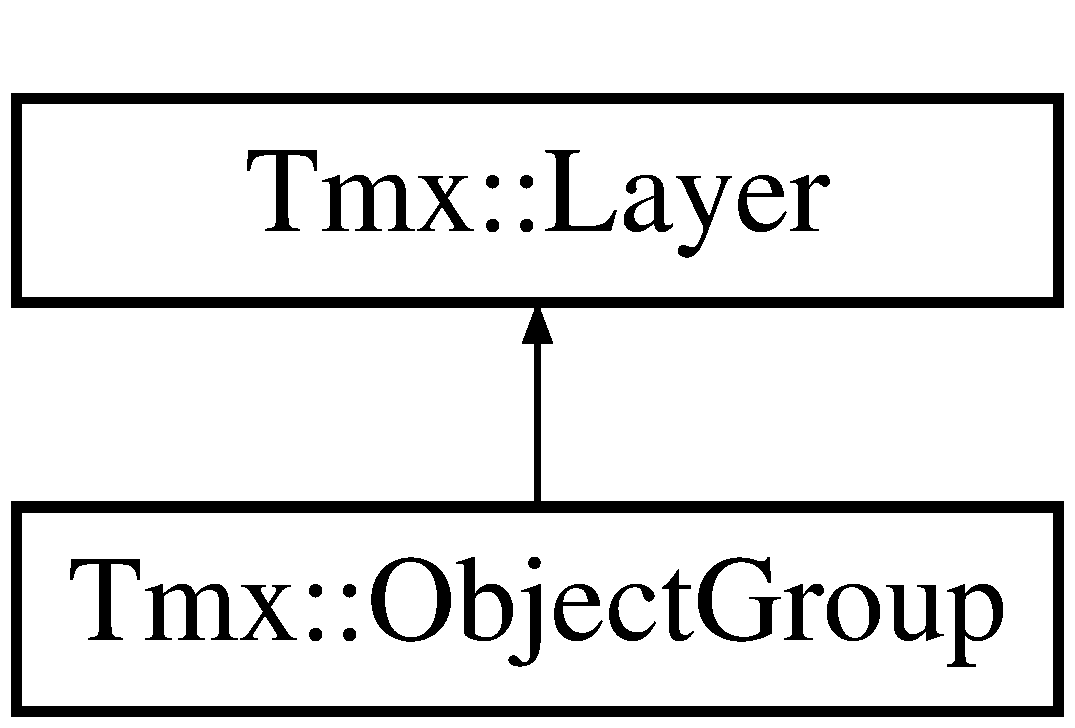
\includegraphics[height=2.000000cm]{classTmx_1_1ObjectGroup}
\end{center}
\end{figure}
\subsection*{Public Member Functions}
\begin{DoxyCompactItemize}
\item 
\hypertarget{classTmx_1_1ObjectGroup_a99d89c89cd3262d19f4e30d6ba04667d}{\hyperlink{classTmx_1_1ObjectGroup_a99d89c89cd3262d19f4e30d6ba04667d}{Object\-Group} (const \hyperlink{classTmx_1_1Map}{Tmx\-::\-Map} $\ast$\-\_\-map)}\label{classTmx_1_1ObjectGroup_a99d89c89cd3262d19f4e30d6ba04667d}

\begin{DoxyCompactList}\small\item\em Construct a new \hyperlink{classTmx_1_1ObjectGroup}{Object\-Group}. \end{DoxyCompactList}\item 
\hypertarget{classTmx_1_1ObjectGroup_a641f391664b74b67a3e46489750589c6}{void \hyperlink{classTmx_1_1ObjectGroup_a641f391664b74b67a3e46489750589c6}{Parse} (const tinyxml2\-::\-X\-M\-L\-Node $\ast$object\-Group\-Node)}\label{classTmx_1_1ObjectGroup_a641f391664b74b67a3e46489750589c6}

\begin{DoxyCompactList}\small\item\em Parse an objectgroup node. \end{DoxyCompactList}\item 
\hypertarget{classTmx_1_1ObjectGroup_a223a60fc76682a7a4a4b4c69fb257395}{const \hyperlink{classTmx_1_1Object}{Tmx\-::\-Object} $\ast$ \hyperlink{classTmx_1_1ObjectGroup_a223a60fc76682a7a4a4b4c69fb257395}{Get\-Object} (int index) const }\label{classTmx_1_1ObjectGroup_a223a60fc76682a7a4a4b4c69fb257395}

\begin{DoxyCompactList}\small\item\em Get a single object. \end{DoxyCompactList}\item 
\hypertarget{classTmx_1_1ObjectGroup_a6e327fa2f4b9e70b526811c50e634aa4}{int \hyperlink{classTmx_1_1ObjectGroup_a6e327fa2f4b9e70b526811c50e634aa4}{Get\-Num\-Objects} () const }\label{classTmx_1_1ObjectGroup_a6e327fa2f4b9e70b526811c50e634aa4}

\begin{DoxyCompactList}\small\item\em Get the number of objects in the list. \end{DoxyCompactList}\item 
\hypertarget{classTmx_1_1ObjectGroup_a67ac49ea10129de947f7fe971727c65f}{\hyperlink{classTmx_1_1Color}{Tmx\-::\-Color} \hyperlink{classTmx_1_1ObjectGroup_a67ac49ea10129de947f7fe971727c65f}{Get\-Color} () const }\label{classTmx_1_1ObjectGroup_a67ac49ea10129de947f7fe971727c65f}

\begin{DoxyCompactList}\small\item\em Get the color used to display the objects in this group. \end{DoxyCompactList}\item 
\hypertarget{classTmx_1_1ObjectGroup_a7581c383af6ed4f4e7d3a4dda3b89c44}{const std\-::vector$<$ \hyperlink{classTmx_1_1Object}{Tmx\-::\-Object} $\ast$ $>$ \& \hyperlink{classTmx_1_1ObjectGroup_a7581c383af6ed4f4e7d3a4dda3b89c44}{Get\-Objects} () const }\label{classTmx_1_1ObjectGroup_a7581c383af6ed4f4e7d3a4dda3b89c44}

\begin{DoxyCompactList}\small\item\em Get the whole list of objects. \end{DoxyCompactList}\end{DoxyCompactItemize}


\subsection{Detailed Description}
A class used for holding a list of objects. 

This class has a property set. 

The documentation for this class was generated from the following files\-:\begin{DoxyCompactItemize}
\item 
/home/travis/build/sainteos/tmxparser/src/Tmx\-Object\-Group.\-h\item 
/home/travis/build/sainteos/tmxparser/src/Tmx\-Object\-Group.\-cpp\end{DoxyCompactItemize}

\hypertarget{structTmx_1_1Point}{\section{Tmx\-:\-:Point Struct Reference}
\label{structTmx_1_1Point}\index{Tmx\-::\-Point@{Tmx\-::\-Point}}
}


Used to store a vertex of a Polygon/\-Polyline.  




{\ttfamily \#include $<$Tmx\-Point.\-h$>$}

\subsection*{Public Attributes}
\begin{DoxyCompactItemize}
\item 
\hypertarget{structTmx_1_1Point_ab819a07e71c9685306d92b0173fc137c}{float \hyperlink{structTmx_1_1Point_ab819a07e71c9685306d92b0173fc137c}{x}}\label{structTmx_1_1Point_ab819a07e71c9685306d92b0173fc137c}

\begin{DoxyCompactList}\small\item\em X coordinate. \end{DoxyCompactList}\item 
\hypertarget{structTmx_1_1Point_af9ce4e615f66858dcf77f1d2026510ba}{float \hyperlink{structTmx_1_1Point_af9ce4e615f66858dcf77f1d2026510ba}{y}}\label{structTmx_1_1Point_af9ce4e615f66858dcf77f1d2026510ba}

\begin{DoxyCompactList}\small\item\em Y coordinate. \end{DoxyCompactList}\end{DoxyCompactItemize}


\subsection{Detailed Description}
Used to store a vertex of a Polygon/\-Polyline. 

The documentation for this struct was generated from the following file\-:\begin{DoxyCompactItemize}
\item 
/home/travis/build/sainteos/tmxparser/src/Tmx\-Point.\-h\end{DoxyCompactItemize}

\hypertarget{classTmx_1_1Polygon}{\section{Tmx\-:\-:Polygon Class Reference}
\label{classTmx_1_1Polygon}\index{Tmx\-::\-Polygon@{Tmx\-::\-Polygon}}
}


Class to store a \hyperlink{classTmx_1_1Polygon}{Polygon} of an \hyperlink{classTmx_1_1Object}{Object}.  




{\ttfamily \#include $<$Tmx\-Polygon.\-h$>$}

\subsection*{Public Member Functions}
\begin{DoxyCompactItemize}
\item 
\hypertarget{classTmx_1_1Polygon_a4d4f38e3f1db96cb02a09636559d63de}{void \hyperlink{classTmx_1_1Polygon_a4d4f38e3f1db96cb02a09636559d63de}{Parse} (const tinyxml2\-::\-X\-M\-L\-Node $\ast$polygon\-Node)}\label{classTmx_1_1Polygon_a4d4f38e3f1db96cb02a09636559d63de}

\begin{DoxyCompactList}\small\item\em Parse the polygon node. \end{DoxyCompactList}\item 
\hypertarget{classTmx_1_1Polygon_aec32fbd6874273145cc874bf0068fe61}{const \hyperlink{structTmx_1_1Point}{Tmx\-::\-Point} \& \hyperlink{classTmx_1_1Polygon_aec32fbd6874273145cc874bf0068fe61}{Get\-Point} (int index) const }\label{classTmx_1_1Polygon_aec32fbd6874273145cc874bf0068fe61}

\begin{DoxyCompactList}\small\item\em Get one of the vertices. \end{DoxyCompactList}\item 
\hypertarget{classTmx_1_1Polygon_a708ce0f1008079468323126549a3108f}{int \hyperlink{classTmx_1_1Polygon_a708ce0f1008079468323126549a3108f}{Get\-Num\-Points} () const }\label{classTmx_1_1Polygon_a708ce0f1008079468323126549a3108f}

\begin{DoxyCompactList}\small\item\em Get the number of vertices. \end{DoxyCompactList}\end{DoxyCompactItemize}


\subsection{Detailed Description}
Class to store a \hyperlink{classTmx_1_1Polygon}{Polygon} of an \hyperlink{classTmx_1_1Object}{Object}. 

The documentation for this class was generated from the following files\-:\begin{DoxyCompactItemize}
\item 
/home/travis/build/sainteos/tmxparser/src/Tmx\-Polygon.\-h\item 
/home/travis/build/sainteos/tmxparser/src/Tmx\-Polygon.\-cpp\end{DoxyCompactItemize}

\hypertarget{classTmx_1_1Polyline}{\section{Tmx\-:\-:Polyline Class Reference}
\label{classTmx_1_1Polyline}\index{Tmx\-::\-Polyline@{Tmx\-::\-Polyline}}
}


Class to store a \hyperlink{classTmx_1_1Polyline}{Polyline} of an \hyperlink{classTmx_1_1Object}{Object}.  




{\ttfamily \#include $<$Tmx\-Polyline.\-h$>$}

\subsection*{Public Member Functions}
\begin{DoxyCompactItemize}
\item 
\hypertarget{classTmx_1_1Polyline_a6accc5ff77af04b4e3e0a70b1bcecaff}{void \hyperlink{classTmx_1_1Polyline_a6accc5ff77af04b4e3e0a70b1bcecaff}{Parse} (const tinyxml2\-::\-X\-M\-L\-Node $\ast$polyline\-Node)}\label{classTmx_1_1Polyline_a6accc5ff77af04b4e3e0a70b1bcecaff}

\begin{DoxyCompactList}\small\item\em Parse the polyline node. \end{DoxyCompactList}\item 
\hypertarget{classTmx_1_1Polyline_a1ec179549019163c7803e959cc6506b6}{const \hyperlink{structTmx_1_1Point}{Tmx\-::\-Point} \& \hyperlink{classTmx_1_1Polyline_a1ec179549019163c7803e959cc6506b6}{Get\-Point} (int index) const }\label{classTmx_1_1Polyline_a1ec179549019163c7803e959cc6506b6}

\begin{DoxyCompactList}\small\item\em Get one of the vertices. \end{DoxyCompactList}\item 
\hypertarget{classTmx_1_1Polyline_a7df0a235f803247a9c756cd3793adfbb}{int \hyperlink{classTmx_1_1Polyline_a7df0a235f803247a9c756cd3793adfbb}{Get\-Num\-Points} () const }\label{classTmx_1_1Polyline_a7df0a235f803247a9c756cd3793adfbb}

\begin{DoxyCompactList}\small\item\em Get the number of vertices. \end{DoxyCompactList}\end{DoxyCompactItemize}


\subsection{Detailed Description}
Class to store a \hyperlink{classTmx_1_1Polyline}{Polyline} of an \hyperlink{classTmx_1_1Object}{Object}. 

The documentation for this class was generated from the following files\-:\begin{DoxyCompactItemize}
\item 
/home/travis/build/sainteos/tmxparser/src/Tmx\-Polyline.\-h\item 
/home/travis/build/sainteos/tmxparser/src/Tmx\-Polyline.\-cpp\end{DoxyCompactItemize}

\hypertarget{classTmx_1_1Property}{\section{Tmx\-:\-:Property Class Reference}
\label{classTmx_1_1Property}\index{Tmx\-::\-Property@{Tmx\-::\-Property}}
}


Used to store a (typed) property.  




{\ttfamily \#include $<$Tmx\-Property.\-h$>$}

\subsection*{Public Member Functions}
\begin{DoxyCompactItemize}
\item 
\hypertarget{classTmx_1_1Property_a3433bfba5413e8a685832361e03d5dd3}{void \hyperlink{classTmx_1_1Property_a3433bfba5413e8a685832361e03d5dd3}{Parse} (const tinyxml2\-::\-X\-M\-L\-Element $\ast$property\-Elem)}\label{classTmx_1_1Property_a3433bfba5413e8a685832361e03d5dd3}

\begin{DoxyCompactList}\small\item\em Parse the property element. \end{DoxyCompactList}\item 
\hypertarget{classTmx_1_1Property_a044e2f2d7b7b6d331df49a0cf5782375}{Property\-Type \hyperlink{classTmx_1_1Property_a044e2f2d7b7b6d331df49a0cf5782375}{Get\-Type} () const }\label{classTmx_1_1Property_a044e2f2d7b7b6d331df49a0cf5782375}

\begin{DoxyCompactList}\small\item\em Get the type of the property (default\-: T\-M\-X\-\_\-\-P\-R\-O\-P\-E\-R\-T\-Y\-\_\-\-S\-T\-R\-I\-N\-G) \end{DoxyCompactList}\item 
\hypertarget{classTmx_1_1Property_ae969a247c4e494c13c15a96fe8f9c227}{bool \hyperlink{classTmx_1_1Property_ae969a247c4e494c13c15a96fe8f9c227}{Is\-Of\-Type} (Property\-Type type) const }\label{classTmx_1_1Property_ae969a247c4e494c13c15a96fe8f9c227}

\begin{DoxyCompactList}\small\item\em Check if the property is of a certain type. \end{DoxyCompactList}\item 
\hypertarget{classTmx_1_1Property_a3e9c675710a0c442ab18a48d070b1f78}{const std\-::string \& \hyperlink{classTmx_1_1Property_a3e9c675710a0c442ab18a48d070b1f78}{Get\-Value} () const }\label{classTmx_1_1Property_a3e9c675710a0c442ab18a48d070b1f78}

\begin{DoxyCompactList}\small\item\em Return the value of the property. \end{DoxyCompactList}\item 
\hypertarget{classTmx_1_1Property_aa5612f8dc82ba4c0a8411adbba618fd0}{bool \hyperlink{classTmx_1_1Property_aa5612f8dc82ba4c0a8411adbba618fd0}{Is\-Value\-Empty} () const }\label{classTmx_1_1Property_aa5612f8dc82ba4c0a8411adbba618fd0}

\begin{DoxyCompactList}\small\item\em Return whether the value is empty or was not specified. \end{DoxyCompactList}\item 
\hypertarget{classTmx_1_1Property_a6d5936badc6223e1d6d8ffc1427e3508}{bool \hyperlink{classTmx_1_1Property_a6d5936badc6223e1d6d8ffc1427e3508}{Get\-Bool\-Value} (bool default\-Value=false) const }\label{classTmx_1_1Property_a6d5936badc6223e1d6d8ffc1427e3508}

\begin{DoxyCompactList}\small\item\em Convert the value to a boolean and return it (or the default value if not a boolean.) \end{DoxyCompactList}\item 
\hypertarget{classTmx_1_1Property_a1007a9ffdf340d29fd5ad5dce1e35c60}{int \hyperlink{classTmx_1_1Property_a1007a9ffdf340d29fd5ad5dce1e35c60}{Get\-Int\-Value} (int default\-Value=0) const }\label{classTmx_1_1Property_a1007a9ffdf340d29fd5ad5dce1e35c60}

\begin{DoxyCompactList}\small\item\em Convert the value to an integer and return it (or the default value if not an integer). \end{DoxyCompactList}\item 
\hypertarget{classTmx_1_1Property_a45b53f91382137b88a9621ebc670881d}{float \hyperlink{classTmx_1_1Property_a45b53f91382137b88a9621ebc670881d}{Get\-Float\-Value} (float default\-Value=0.\-0f) const }\label{classTmx_1_1Property_a45b53f91382137b88a9621ebc670881d}

\begin{DoxyCompactList}\small\item\em Convert the value to a float and return it (or the default value if not a float). \end{DoxyCompactList}\item 
\hypertarget{classTmx_1_1Property_a8cdbef1757c46929ae796c6761422b5a}{\hyperlink{classTmx_1_1Color}{Tmx\-::\-Color} \hyperlink{classTmx_1_1Property_a8cdbef1757c46929ae796c6761422b5a}{Get\-Color\-Value} (\hyperlink{classTmx_1_1Color}{Tmx\-::\-Color} default\-Value=\hyperlink{classTmx_1_1Color}{Tmx\-::\-Color}()) const }\label{classTmx_1_1Property_a8cdbef1757c46929ae796c6761422b5a}

\begin{DoxyCompactList}\small\item\em Convert the value to a color and return it (or the default value if not a color). \end{DoxyCompactList}\end{DoxyCompactItemize}


\subsection{Detailed Description}
Used to store a (typed) property. 

The documentation for this class was generated from the following files\-:\begin{DoxyCompactItemize}
\item 
/home/travis/build/sainteos/tmxparser/src/Tmx\-Property.\-h\item 
/home/travis/build/sainteos/tmxparser/src/Tmx\-Property.\-cpp\end{DoxyCompactItemize}

\hypertarget{classTmx_1_1PropertySet}{\section{Tmx\-:\-:Property\-Set Class Reference}
\label{classTmx_1_1PropertySet}\index{Tmx\-::\-Property\-Set@{Tmx\-::\-Property\-Set}}
}


This class contains a map of properties.  




{\ttfamily \#include $<$Tmx\-Property\-Set.\-h$>$}

\subsection*{Public Member Functions}
\begin{DoxyCompactItemize}
\item 
\hypertarget{classTmx_1_1PropertySet_a242a55171b6dff9be49aa27fc157fec2}{void \hyperlink{classTmx_1_1PropertySet_a242a55171b6dff9be49aa27fc157fec2}{Parse} (const tinyxml2\-::\-X\-M\-L\-Node $\ast$properties\-Node)}\label{classTmx_1_1PropertySet_a242a55171b6dff9be49aa27fc157fec2}

\begin{DoxyCompactList}\small\item\em Parse a node containing all the property nodes. \end{DoxyCompactList}\item 
\hypertarget{classTmx_1_1PropertySet_ac83515f6a70328784ff88a7c95fc095c}{int \hyperlink{classTmx_1_1PropertySet_ac83515f6a70328784ff88a7c95fc095c}{Get\-Int\-Property} (const std\-::string \&name, int default\-Value=0) const }\label{classTmx_1_1PropertySet_ac83515f6a70328784ff88a7c95fc095c}

\begin{DoxyCompactList}\small\item\em Get a int property. \end{DoxyCompactList}\item 
\hypertarget{classTmx_1_1PropertySet_a5cda9c71a56fada3c938e3be1cf64a91}{float \hyperlink{classTmx_1_1PropertySet_a5cda9c71a56fada3c938e3be1cf64a91}{Get\-Float\-Property} (const std\-::string \&name, float default\-Value=0.\-0f) const }\label{classTmx_1_1PropertySet_a5cda9c71a56fada3c938e3be1cf64a91}

\begin{DoxyCompactList}\small\item\em Get a float property. \end{DoxyCompactList}\item 
\hypertarget{classTmx_1_1PropertySet_a307ae6b1427fba22a9304bf8ad1ef946}{std\-::string \hyperlink{classTmx_1_1PropertySet_a307ae6b1427fba22a9304bf8ad1ef946}{Get\-String\-Property} (const std\-::string \&name, std\-::string default\-Value=\char`\"{}\char`\"{}) const }\label{classTmx_1_1PropertySet_a307ae6b1427fba22a9304bf8ad1ef946}

\begin{DoxyCompactList}\small\item\em Get a string property. \end{DoxyCompactList}\item 
\hypertarget{classTmx_1_1PropertySet_a0ba8ecdf58e289e2dee57ce38b9df20d}{bool \hyperlink{classTmx_1_1PropertySet_a0ba8ecdf58e289e2dee57ce38b9df20d}{Get\-Bool\-Property} (const std\-::string \&name, bool default\-Value=false) const }\label{classTmx_1_1PropertySet_a0ba8ecdf58e289e2dee57ce38b9df20d}

\begin{DoxyCompactList}\small\item\em Get a bool property. \end{DoxyCompactList}\item 
\hypertarget{classTmx_1_1PropertySet_a02fb8f1bc34d169cc5a8fd148360c915}{\hyperlink{classTmx_1_1Color}{Tmx\-::\-Color} \hyperlink{classTmx_1_1PropertySet_a02fb8f1bc34d169cc5a8fd148360c915}{Get\-Color\-Property} (const std\-::string \&name, \hyperlink{classTmx_1_1Color}{Tmx\-::\-Color} default\-Value=\hyperlink{classTmx_1_1Color}{Tmx\-::\-Color}()) const }\label{classTmx_1_1PropertySet_a02fb8f1bc34d169cc5a8fd148360c915}

\begin{DoxyCompactList}\small\item\em Get a color property. \end{DoxyCompactList}\item 
\hypertarget{classTmx_1_1PropertySet_a67b47b4e15e8df963911c798f792a2cc}{int \hyperlink{classTmx_1_1PropertySet_a67b47b4e15e8df963911c798f792a2cc}{Get\-Size} () const }\label{classTmx_1_1PropertySet_a67b47b4e15e8df963911c798f792a2cc}

\begin{DoxyCompactList}\small\item\em Returns the amount of properties. \end{DoxyCompactList}\item 
\hypertarget{classTmx_1_1PropertySet_a9581ebb5a9683662887151f1e92b664a}{bool \hyperlink{classTmx_1_1PropertySet_a9581ebb5a9683662887151f1e92b664a}{Has\-Property} (const std\-::string \&name) const }\label{classTmx_1_1PropertySet_a9581ebb5a9683662887151f1e92b664a}

\begin{DoxyCompactList}\small\item\em Checks if a property exists in the set. \end{DoxyCompactList}\item 
\hypertarget{classTmx_1_1PropertySet_a459999829fc14e72decdd60e378d0531}{const std\-::unordered\-\_\-map\\*
$<$ std\-::string, \hyperlink{classTmx_1_1Property}{Property} $>$ \& \hyperlink{classTmx_1_1PropertySet_a459999829fc14e72decdd60e378d0531}{Get\-Property\-Map} () const }\label{classTmx_1_1PropertySet_a459999829fc14e72decdd60e378d0531}

\begin{DoxyCompactList}\small\item\em Returns the unordered map of properties. \end{DoxyCompactList}\item 
std\-::map$<$ std\-::string, \\*
std\-::string $>$ \hyperlink{classTmx_1_1PropertySet_aa8929cdbcf9fc7a767ee98c33ab3130c}{Get\-List} () const 
\begin{DoxyCompactList}\small\item\em Returns the S\-T\-L map of the properties. \end{DoxyCompactList}\item 
\hypertarget{classTmx_1_1PropertySet_a5a107beb5e2dfc94dc61dfaa2abc1716}{bool \hyperlink{classTmx_1_1PropertySet_a5a107beb5e2dfc94dc61dfaa2abc1716}{Empty} () const }\label{classTmx_1_1PropertySet_a5a107beb5e2dfc94dc61dfaa2abc1716}

\begin{DoxyCompactList}\small\item\em Returns whether there are no properties. \end{DoxyCompactList}\end{DoxyCompactItemize}


\subsection{Detailed Description}
This class contains a map of properties. 

\subsection{Member Function Documentation}
\hypertarget{classTmx_1_1PropertySet_aa8929cdbcf9fc7a767ee98c33ab3130c}{\index{Tmx\-::\-Property\-Set@{Tmx\-::\-Property\-Set}!Get\-List@{Get\-List}}
\index{Get\-List@{Get\-List}!Tmx::PropertySet@{Tmx\-::\-Property\-Set}}
\subsubsection[{Get\-List}]{\setlength{\rightskip}{0pt plus 5cm}std\-::map$<$ std\-::string, std\-::string $>$ Tmx\-::\-Property\-Set\-::\-Get\-List (
\begin{DoxyParamCaption}
{}
\end{DoxyParamCaption}
) const}}\label{classTmx_1_1PropertySet_aa8929cdbcf9fc7a767ee98c33ab3130c}


Returns the S\-T\-L map of the properties. 

Deprecated, please use \hyperlink{classTmx_1_1PropertySet_a459999829fc14e72decdd60e378d0531}{Get\-Property\-Map()} instead. 

The documentation for this class was generated from the following files\-:\begin{DoxyCompactItemize}
\item 
/home/travis/build/sainteos/tmxparser/src/Tmx\-Property\-Set.\-h\item 
/home/travis/build/sainteos/tmxparser/src/Tmx\-Property\-Set.\-cpp\end{DoxyCompactItemize}

\hypertarget{classTmx_1_1Terrain}{\section{Tmx\-:\-:Terrain Class Reference}
\label{classTmx_1_1Terrain}\index{Tmx\-::\-Terrain@{Tmx\-::\-Terrain}}
}


Class to contain information about every terrain in the tileset/terraintypes element.  




{\ttfamily \#include $<$Tmx\-Terrain.\-h$>$}

\subsection*{Public Member Functions}
\begin{DoxyCompactItemize}
\item 
\hypertarget{classTmx_1_1Terrain_afe30f92af38023bf56adc2ae8f8e580d}{void \hyperlink{classTmx_1_1Terrain_afe30f92af38023bf56adc2ae8f8e580d}{Parse} (const tinyxml2\-::\-X\-M\-L\-Node $\ast$terrain\-Node)}\label{classTmx_1_1Terrain_afe30f92af38023bf56adc2ae8f8e580d}

\begin{DoxyCompactList}\small\item\em Parse a terrain type node. \end{DoxyCompactList}\item 
\hypertarget{classTmx_1_1Terrain_a623a166c19f3c33d7b80d3c435fdf1ac}{const std\-::string \& \hyperlink{classTmx_1_1Terrain_a623a166c19f3c33d7b80d3c435fdf1ac}{Get\-Name} () const }\label{classTmx_1_1Terrain_a623a166c19f3c33d7b80d3c435fdf1ac}

\begin{DoxyCompactList}\small\item\em Get the name of the terrain type. \end{DoxyCompactList}\item 
\hypertarget{classTmx_1_1Terrain_a20ecd6765c02f84bc51656bf0681bcb6}{int \hyperlink{classTmx_1_1Terrain_a20ecd6765c02f84bc51656bf0681bcb6}{Get\-Tile\-Id} () const }\label{classTmx_1_1Terrain_a20ecd6765c02f84bc51656bf0681bcb6}

\begin{DoxyCompactList}\small\item\em Get the local tile-\/id of the tile that represents the terrain type visually. \end{DoxyCompactList}\item 
\hypertarget{classTmx_1_1Terrain_a2bb5f2870d2e94e9c7472fc700a94ee5}{const \hyperlink{classTmx_1_1PropertySet}{Tmx\-::\-Property\-Set} \& \hyperlink{classTmx_1_1Terrain_a2bb5f2870d2e94e9c7472fc700a94ee5}{Get\-Properties} () const }\label{classTmx_1_1Terrain_a2bb5f2870d2e94e9c7472fc700a94ee5}

\begin{DoxyCompactList}\small\item\em Get a set of properties regarding the terrain type. \end{DoxyCompactList}\end{DoxyCompactItemize}


\subsection{Detailed Description}
Class to contain information about every terrain in the tileset/terraintypes element. 

This class also contains a property set. 

The documentation for this class was generated from the following files\-:\begin{DoxyCompactItemize}
\item 
/home/travis/build/sainteos/tmxparser/src/Tmx\-Terrain.\-h\item 
/home/travis/build/sainteos/tmxparser/src/Tmx\-Terrain.\-cpp\end{DoxyCompactItemize}

\hypertarget{classTmx_1_1TerrainArray}{\section{Tmx\-:\-:Terrain\-Array Class Reference}
\label{classTmx_1_1TerrainArray}\index{Tmx\-::\-Terrain\-Array@{Tmx\-::\-Terrain\-Array}}
}


Class to parse terrain types, which can be referenced from the terrain attribute of the tileset/tile element.  




{\ttfamily \#include $<$Tmx\-Terrain\-Array.\-h$>$}

\subsection*{Public Member Functions}
\begin{DoxyCompactItemize}
\item 
\hypertarget{classTmx_1_1TerrainArray_a95f03506b503efef05703db89dfff16e}{void \hyperlink{classTmx_1_1TerrainArray_a95f03506b503efef05703db89dfff16e}{Parse} (std\-::vector$<$ \hyperlink{classTmx_1_1Terrain}{Tmx\-::\-Terrain} $\ast$ $>$ $\ast$terrain\-Types, const tinyxml2\-::\-X\-M\-L\-Node $\ast$terrain\-Array\-Node)}\label{classTmx_1_1TerrainArray_a95f03506b503efef05703db89dfff16e}

\begin{DoxyCompactList}\small\item\em Parse a node containing all the terrain nodes. \end{DoxyCompactList}\end{DoxyCompactItemize}


\subsection{Detailed Description}
Class to parse terrain types, which can be referenced from the terrain attribute of the tileset/tile element. 



The documentation for this class was generated from the following files\-:\begin{DoxyCompactItemize}
\item 
/home/travis/build/sainteos/tmxparser/src/Tmx\-Terrain\-Array.\-h\item 
/home/travis/build/sainteos/tmxparser/src/Tmx\-Terrain\-Array.\-cpp\end{DoxyCompactItemize}

\hypertarget{classTmx_1_1Tile}{\section{Tmx\-:\-:Tile Class Reference}
\label{classTmx_1_1Tile}\index{Tmx\-::\-Tile@{Tmx\-::\-Tile}}
}


Class to contain information about every tile in the tileset/tiles element.  




{\ttfamily \#include $<$Tmx\-Tile.\-h$>$}

\subsection*{Public Member Functions}
\begin{DoxyCompactItemize}
\item 
\hypertarget{classTmx_1_1Tile_ae3320f562455e8a92879c18aaae353ac}{\hyperlink{classTmx_1_1Tile_ae3320f562455e8a92879c18aaae353ac}{Tile} (int id)}\label{classTmx_1_1Tile_ae3320f562455e8a92879c18aaae353ac}

\begin{DoxyCompactList}\small\item\em Construct a new tile with the given id. \end{DoxyCompactList}\item 
\hypertarget{classTmx_1_1Tile_a488334cb54d1d5735f636eb3b198d901}{void \hyperlink{classTmx_1_1Tile_a488334cb54d1d5735f636eb3b198d901}{Parse} (const tinyxml2\-::\-X\-M\-L\-Node $\ast$tile\-Node)}\label{classTmx_1_1Tile_a488334cb54d1d5735f636eb3b198d901}

\begin{DoxyCompactList}\small\item\em Parse a tile node. \end{DoxyCompactList}\item 
\hypertarget{classTmx_1_1Tile_a5b8c40fa159f3e52e8f74a2fa8a17b1f}{int \hyperlink{classTmx_1_1Tile_a5b8c40fa159f3e52e8f74a2fa8a17b1f}{Get\-Id} () const }\label{classTmx_1_1Tile_a5b8c40fa159f3e52e8f74a2fa8a17b1f}

\begin{DoxyCompactList}\small\item\em Get the Id. (relative to the tileset) \end{DoxyCompactList}\item 
\hypertarget{classTmx_1_1Tile_ab8993fd3a43772a14d78c0ae9a142f2a}{bool \hyperlink{classTmx_1_1Tile_ab8993fd3a43772a14d78c0ae9a142f2a}{Is\-Animated} () const }\label{classTmx_1_1Tile_ab8993fd3a43772a14d78c0ae9a142f2a}

\begin{DoxyCompactList}\small\item\em Returns true if the tile is animated (has one or more animation frames) \end{DoxyCompactList}\item 
\hypertarget{classTmx_1_1Tile_a622a7fd2afa260652aed512e09e988dc}{int \hyperlink{classTmx_1_1Tile_a622a7fd2afa260652aed512e09e988dc}{Get\-Frame\-Count} () const }\label{classTmx_1_1Tile_a622a7fd2afa260652aed512e09e988dc}

\begin{DoxyCompactList}\small\item\em Returns the number of frames of the animation. If the tile is not animated, returns 0. \end{DoxyCompactList}\item 
unsigned int \hyperlink{classTmx_1_1Tile_a06cd238d0fd53822ef1487498a890944}{Get\-Total\-Duration} () const 
\begin{DoxyCompactList}\small\item\em Returns the total duration of the animation, in milliseconds, or 0 if the tile is not animated. \end{DoxyCompactList}\item 
\hypertarget{classTmx_1_1Tile_aa7a6ad2d344f32f88e1a88c06edc4c3f}{const \hyperlink{classTmx_1_1Image}{Tmx\-::\-Image} $\ast$ \hyperlink{classTmx_1_1Tile_aa7a6ad2d344f32f88e1a88c06edc4c3f}{Get\-Image} () const }\label{classTmx_1_1Tile_aa7a6ad2d344f32f88e1a88c06edc4c3f}

\begin{DoxyCompactList}\small\item\em Retrurns the tile image if defined. \end{DoxyCompactList}\item 
\hypertarget{classTmx_1_1Tile_af46d006ea914db476b90d0866a12564d}{const std\-::vector\\*
$<$ \hyperlink{classTmx_1_1AnimationFrame}{Animation\-Frame} $>$ \& \hyperlink{classTmx_1_1Tile_af46d006ea914db476b90d0866a12564d}{Get\-Frames} () const }\label{classTmx_1_1Tile_af46d006ea914db476b90d0866a12564d}

\begin{DoxyCompactList}\small\item\em Returns the frames of the animation. \end{DoxyCompactList}\item 
\hypertarget{classTmx_1_1Tile_aa5cc1be340fa012e16c6ed62fb84f908}{const \hyperlink{classTmx_1_1PropertySet}{Tmx\-::\-Property\-Set} \& \hyperlink{classTmx_1_1Tile_aa5cc1be340fa012e16c6ed62fb84f908}{Get\-Properties} () const }\label{classTmx_1_1Tile_aa5cc1be340fa012e16c6ed62fb84f908}

\begin{DoxyCompactList}\small\item\em Get a set of properties regarding the tile. \end{DoxyCompactList}\item 
\hypertarget{classTmx_1_1Tile_a8b0aee9d016fbb3c912b0ac7153a2333}{std\-::vector$<$ \hyperlink{classTmx_1_1Object}{Tmx\-::\-Object} $\ast$ $>$ \hyperlink{classTmx_1_1Tile_a8b0aee9d016fbb3c912b0ac7153a2333}{Get\-Objects} () const }\label{classTmx_1_1Tile_a8b0aee9d016fbb3c912b0ac7153a2333}

\begin{DoxyCompactList}\small\item\em Get set of Collision Objects. \end{DoxyCompactList}\item 
\hypertarget{classTmx_1_1Tile_a31a59f592e9a2ec96b57aa77eca98bf3}{bool \hyperlink{classTmx_1_1Tile_a31a59f592e9a2ec96b57aa77eca98bf3}{Has\-Objects} () const }\label{classTmx_1_1Tile_a31a59f592e9a2ec96b57aa77eca98bf3}

\begin{DoxyCompactList}\small\item\em Returns true if tile has Collision Objects. \end{DoxyCompactList}\item 
\hypertarget{classTmx_1_1Tile_a4086d0b8b91fa9e27c3d3f710c7ad50e}{const \hyperlink{classTmx_1_1Object}{Tmx\-::\-Object} $\ast$ \hyperlink{classTmx_1_1Tile_a4086d0b8b91fa9e27c3d3f710c7ad50e}{Get\-Object} (int index) const }\label{classTmx_1_1Tile_a4086d0b8b91fa9e27c3d3f710c7ad50e}

\begin{DoxyCompactList}\small\item\em Get a single object. \end{DoxyCompactList}\item 
\hypertarget{classTmx_1_1Tile_add455b756c2ed715c03aada301d9e5c9}{int \hyperlink{classTmx_1_1Tile_add455b756c2ed715c03aada301d9e5c9}{Get\-Num\-Objects} () const }\label{classTmx_1_1Tile_add455b756c2ed715c03aada301d9e5c9}

\begin{DoxyCompactList}\small\item\em Get the number of objects in the list. \end{DoxyCompactList}\end{DoxyCompactItemize}


\subsection{Detailed Description}
Class to contain information about every tile in the tileset/tiles element. 

It may expand if there are more elements or attributes added into the the tile element. This class also contains a property set. 

\subsection{Member Function Documentation}
\hypertarget{classTmx_1_1Tile_a06cd238d0fd53822ef1487498a890944}{\index{Tmx\-::\-Tile@{Tmx\-::\-Tile}!Get\-Total\-Duration@{Get\-Total\-Duration}}
\index{Get\-Total\-Duration@{Get\-Total\-Duration}!Tmx::Tile@{Tmx\-::\-Tile}}
\subsubsection[{Get\-Total\-Duration}]{\setlength{\rightskip}{0pt plus 5cm}unsigned int Tmx\-::\-Tile\-::\-Get\-Total\-Duration (
\begin{DoxyParamCaption}
{}
\end{DoxyParamCaption}
) const\hspace{0.3cm}{\ttfamily [inline]}}}\label{classTmx_1_1Tile_a06cd238d0fd53822ef1487498a890944}


Returns the total duration of the animation, in milliseconds, or 0 if the tile is not animated. 



The documentation for this class was generated from the following files\-:\begin{DoxyCompactItemize}
\item 
/home/travis/build/sainteos/tmxparser/src/Tmx\-Tile.\-h\item 
/home/travis/build/sainteos/tmxparser/src/Tmx\-Tile.\-cpp\end{DoxyCompactItemize}

\hypertarget{classTmx_1_1TileLayer}{\section{Tmx\-:\-:Tile\-Layer Class Reference}
\label{classTmx_1_1TileLayer}\index{Tmx\-::\-Tile\-Layer@{Tmx\-::\-Tile\-Layer}}
}


Used for storing information about the tile ids for every tile layer.  




{\ttfamily \#include $<$Tmx\-Tile\-Layer.\-h$>$}

Inheritance diagram for Tmx\-:\-:Tile\-Layer\-:\begin{figure}[H]
\begin{center}
\leavevmode
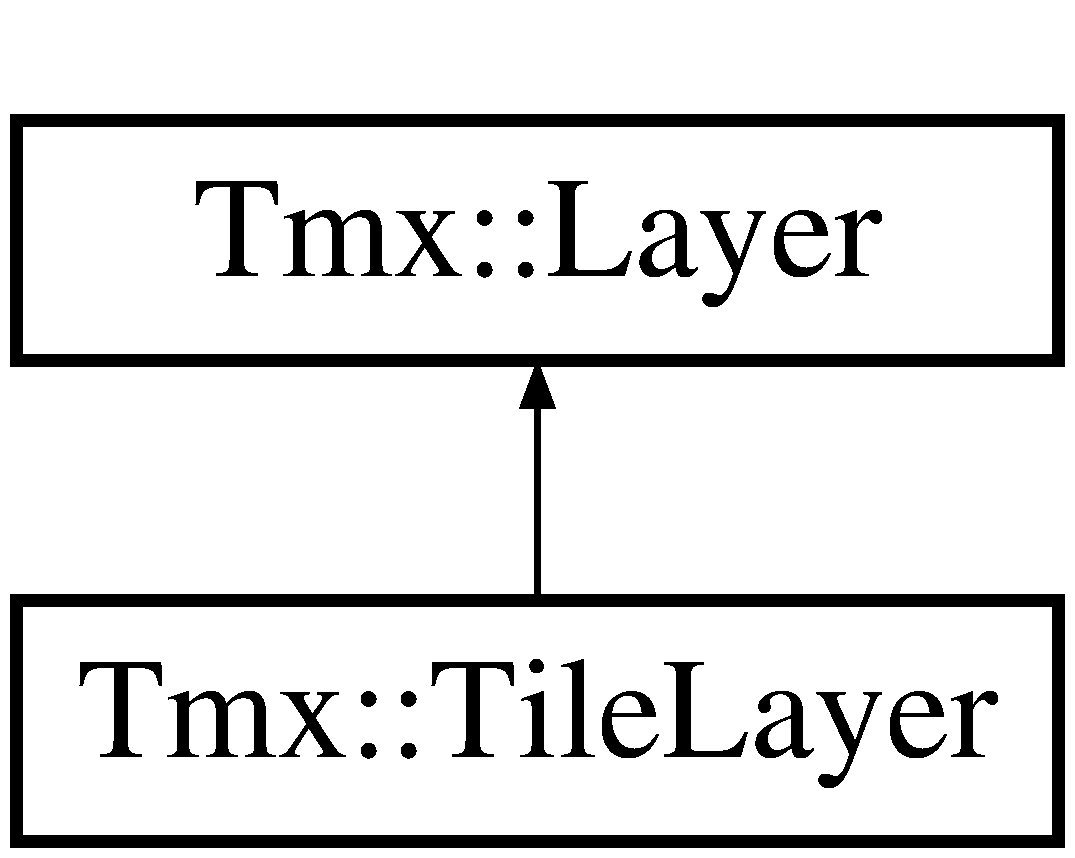
\includegraphics[height=2.000000cm]{classTmx_1_1TileLayer}
\end{center}
\end{figure}
\subsection*{Public Member Functions}
\begin{DoxyCompactItemize}
\item 
\hypertarget{classTmx_1_1TileLayer_a695c876d416b231bd66e19266dd64f08}{\hyperlink{classTmx_1_1TileLayer_a695c876d416b231bd66e19266dd64f08}{Tile\-Layer} (const \hyperlink{classTmx_1_1Map}{Tmx\-::\-Map} $\ast$\-\_\-map)}\label{classTmx_1_1TileLayer_a695c876d416b231bd66e19266dd64f08}

\begin{DoxyCompactList}\small\item\em Construct a \hyperlink{classTmx_1_1TileLayer}{Tile\-Layer} on the given map. \end{DoxyCompactList}\item 
\hypertarget{classTmx_1_1TileLayer_abd369d79635deab99dc03182a49e5d78}{void \hyperlink{classTmx_1_1TileLayer_abd369d79635deab99dc03182a49e5d78}{Parse} (const tinyxml2\-::\-X\-M\-L\-Node $\ast$tile\-Layer\-Node)}\label{classTmx_1_1TileLayer_abd369d79635deab99dc03182a49e5d78}

\begin{DoxyCompactList}\small\item\em Parse a tile layer node. \end{DoxyCompactList}\item 
\hypertarget{classTmx_1_1TileLayer_ae3902bf98b97d38f81a44cc634177042}{unsigned \hyperlink{classTmx_1_1TileLayer_ae3902bf98b97d38f81a44cc634177042}{Get\-Tile\-Id} (int x, int y) const }\label{classTmx_1_1TileLayer_ae3902bf98b97d38f81a44cc634177042}

\begin{DoxyCompactList}\small\item\em Pick a specific tile id from the list. \end{DoxyCompactList}\item 
\hypertarget{classTmx_1_1TileLayer_a5ca43217676bfb8b5f45847587dc4318}{unsigned \hyperlink{classTmx_1_1TileLayer_a5ca43217676bfb8b5f45847587dc4318}{Get\-Tile\-Gid} (int x, int y) const }\label{classTmx_1_1TileLayer_a5ca43217676bfb8b5f45847587dc4318}

\begin{DoxyCompactList}\small\item\em Pick a specific tile gid from the list. \end{DoxyCompactList}\item 
\hypertarget{classTmx_1_1TileLayer_a3317d70d127a4f1c3101a61f4c38b100}{int \hyperlink{classTmx_1_1TileLayer_a3317d70d127a4f1c3101a61f4c38b100}{Get\-Tile\-Tileset\-Index} (int x, int y) const }\label{classTmx_1_1TileLayer_a3317d70d127a4f1c3101a61f4c38b100}

\begin{DoxyCompactList}\small\item\em Get the tileset index for a tileset from the list. \end{DoxyCompactList}\item 
\hypertarget{classTmx_1_1TileLayer_a65cf0f77fcebdb13a4d8a58f6af35634}{bool \hyperlink{classTmx_1_1TileLayer_a65cf0f77fcebdb13a4d8a58f6af35634}{Is\-Tile\-Flipped\-Horizontally} (int x, int y) const }\label{classTmx_1_1TileLayer_a65cf0f77fcebdb13a4d8a58f6af35634}

\begin{DoxyCompactList}\small\item\em Get whether a tile is flipped horizontally. \end{DoxyCompactList}\item 
\hypertarget{classTmx_1_1TileLayer_a318e88a21c62a5bc642162dcc0b880c8}{bool \hyperlink{classTmx_1_1TileLayer_a318e88a21c62a5bc642162dcc0b880c8}{Is\-Tile\-Flipped\-Vertically} (int x, int y) const }\label{classTmx_1_1TileLayer_a318e88a21c62a5bc642162dcc0b880c8}

\begin{DoxyCompactList}\small\item\em Get whether a tile is flipped vertically. \end{DoxyCompactList}\item 
\hypertarget{classTmx_1_1TileLayer_a151af08626fb9edee291dc20f431c130}{bool \hyperlink{classTmx_1_1TileLayer_a151af08626fb9edee291dc20f431c130}{Is\-Tile\-Flipped\-Diagonally} (int x, int y) const }\label{classTmx_1_1TileLayer_a151af08626fb9edee291dc20f431c130}

\begin{DoxyCompactList}\small\item\em Get whether a tile is flipped diagonally. \end{DoxyCompactList}\item 
\hypertarget{classTmx_1_1TileLayer_aa945617d235b87e9b532ddcad2f88af0}{const \hyperlink{structTmx_1_1MapTile}{Tmx\-::\-Map\-Tile} \& \hyperlink{classTmx_1_1TileLayer_aa945617d235b87e9b532ddcad2f88af0}{Get\-Tile} (int x, int y) const }\label{classTmx_1_1TileLayer_aa945617d235b87e9b532ddcad2f88af0}

\begin{DoxyCompactList}\small\item\em Get the tile at the given position. \end{DoxyCompactList}\item 
\hypertarget{classTmx_1_1TileLayer_a26aa35c451cdca8dce826167717280e0}{const \hyperlink{structTmx_1_1MapTile}{Tmx\-::\-Map\-Tile} \& \hyperlink{classTmx_1_1TileLayer_a26aa35c451cdca8dce826167717280e0}{Get\-Tile} (int index) const }\label{classTmx_1_1TileLayer_a26aa35c451cdca8dce826167717280e0}

\begin{DoxyCompactList}\small\item\em Get a tile by its index. \end{DoxyCompactList}\item 
Tmx\-::\-Tile\-Layer\-Encoding\-Type \hyperlink{classTmx_1_1TileLayer_a7781153483bb3e1c8928dab0503b3bda}{Get\-Encoding} () const 
\begin{DoxyCompactList}\small\item\em Get the type of encoding that was used for parsing the tile layer data. \end{DoxyCompactList}\item 
Tmx\-::\-Tile\-Layer\-Compression\-Type \hyperlink{classTmx_1_1TileLayer_a94a5548e7784fb064179d7164ae563ce}{Get\-Compression} () const 
\begin{DoxyCompactList}\small\item\em Get the type of compression that was used for parsing the tile layer data. \end{DoxyCompactList}\end{DoxyCompactItemize}


\subsection{Detailed Description}
Used for storing information about the tile ids for every tile layer. 

This class also have a property set. 

\subsection{Member Function Documentation}
\hypertarget{classTmx_1_1TileLayer_a94a5548e7784fb064179d7164ae563ce}{\index{Tmx\-::\-Tile\-Layer@{Tmx\-::\-Tile\-Layer}!Get\-Compression@{Get\-Compression}}
\index{Get\-Compression@{Get\-Compression}!Tmx::TileLayer@{Tmx\-::\-Tile\-Layer}}
\subsubsection[{Get\-Compression}]{\setlength{\rightskip}{0pt plus 5cm}Tmx\-::\-Tile\-Layer\-Compression\-Type Tmx\-::\-Tile\-Layer\-::\-Get\-Compression (
\begin{DoxyParamCaption}
{}
\end{DoxyParamCaption}
) const\hspace{0.3cm}{\ttfamily [inline]}}}\label{classTmx_1_1TileLayer_a94a5548e7784fb064179d7164ae563ce}


Get the type of compression that was used for parsing the tile layer data. 

See\-: Tile\-Layer\-Compression\-Type \hypertarget{classTmx_1_1TileLayer_a7781153483bb3e1c8928dab0503b3bda}{\index{Tmx\-::\-Tile\-Layer@{Tmx\-::\-Tile\-Layer}!Get\-Encoding@{Get\-Encoding}}
\index{Get\-Encoding@{Get\-Encoding}!Tmx::TileLayer@{Tmx\-::\-Tile\-Layer}}
\subsubsection[{Get\-Encoding}]{\setlength{\rightskip}{0pt plus 5cm}Tmx\-::\-Tile\-Layer\-Encoding\-Type Tmx\-::\-Tile\-Layer\-::\-Get\-Encoding (
\begin{DoxyParamCaption}
{}
\end{DoxyParamCaption}
) const\hspace{0.3cm}{\ttfamily [inline]}}}\label{classTmx_1_1TileLayer_a7781153483bb3e1c8928dab0503b3bda}


Get the type of encoding that was used for parsing the tile layer data. 

See\-: Tile\-Layer\-Encoding\-Type 

The documentation for this class was generated from the following files\-:\begin{DoxyCompactItemize}
\item 
/home/travis/build/sainteos/tmxparser/src/Tmx\-Tile\-Layer.\-h\item 
/home/travis/build/sainteos/tmxparser/src/Tmx\-Tile\-Layer.\-cpp\end{DoxyCompactItemize}

\hypertarget{classTmx_1_1TileOffset}{\section{Tmx\-:\-:Tile\-Offset Class Reference}
\label{classTmx_1_1TileOffset}\index{Tmx\-::\-Tile\-Offset@{Tmx\-::\-Tile\-Offset}}
}


A class used for used to specify an offset in pixels, to be applied when drawing a tile from the related tileset.  




{\ttfamily \#include $<$Tmx\-Tile\-Offset.\-h$>$}

\subsection*{Public Member Functions}
\begin{DoxyCompactItemize}
\item 
\hypertarget{classTmx_1_1TileOffset_aa3efdc7be635e7ea4aebce9f04198a30}{void \hyperlink{classTmx_1_1TileOffset_aa3efdc7be635e7ea4aebce9f04198a30}{Parse} (const tinyxml2\-::\-X\-M\-L\-Node $\ast$tile\-Offset\-Node)}\label{classTmx_1_1TileOffset_aa3efdc7be635e7ea4aebce9f04198a30}

\begin{DoxyCompactList}\small\item\em Parses a tileoffset element. \end{DoxyCompactList}\item 
\hypertarget{classTmx_1_1TileOffset_a7488905c51bb9516609e256838e61a95}{int \hyperlink{classTmx_1_1TileOffset_a7488905c51bb9516609e256838e61a95}{Get\-X} () const }\label{classTmx_1_1TileOffset_a7488905c51bb9516609e256838e61a95}

\begin{DoxyCompactList}\small\item\em Get the value of the x attribute of the tile offset. Horizontal offset in pixels. \end{DoxyCompactList}\item 
\hypertarget{classTmx_1_1TileOffset_aa17366bd769a6c807c1ca8d5b02581f0}{int \hyperlink{classTmx_1_1TileOffset_aa17366bd769a6c807c1ca8d5b02581f0}{Get\-Y} () const }\label{classTmx_1_1TileOffset_aa17366bd769a6c807c1ca8d5b02581f0}

\begin{DoxyCompactList}\small\item\em Get the value of the y attribute of the tile offset. Vertical offset in pixels (positive is down). \end{DoxyCompactList}\end{DoxyCompactItemize}


\subsection{Detailed Description}
A class used for used to specify an offset in pixels, to be applied when drawing a tile from the related tileset. 

When not present, no offset is applied. 

The documentation for this class was generated from the following files\-:\begin{DoxyCompactItemize}
\item 
/home/travis/build/sainteos/tmxparser/src/Tmx\-Tile\-Offset.\-h\item 
/home/travis/build/sainteos/tmxparser/src/Tmx\-Tile\-Offset.\-cpp\end{DoxyCompactItemize}

\hypertarget{classTmx_1_1Tileset}{\section{Tmx\-:\-:Tileset Class Reference}
\label{classTmx_1_1Tileset}\index{Tmx\-::\-Tileset@{Tmx\-::\-Tileset}}
}


A class used for storing information about each of the tilesets.  




{\ttfamily \#include $<$Tmx\-Tileset.\-h$>$}

\subsection*{Public Member Functions}
\begin{DoxyCompactItemize}
\item 
\hypertarget{classTmx_1_1Tileset_a221d83fe8974273d5ae449781a72eda7}{void \hyperlink{classTmx_1_1Tileset_a221d83fe8974273d5ae449781a72eda7}{Parse} (const tinyxml2\-::\-X\-M\-L\-Node $\ast$tileset\-Node, const std\-::string \&file\-\_\-path)}\label{classTmx_1_1Tileset_a221d83fe8974273d5ae449781a72eda7}

\begin{DoxyCompactList}\small\item\em Parse a tileset element. \end{DoxyCompactList}\item 
\hypertarget{classTmx_1_1Tileset_a8fffad2d93e4940d8207a391defcab9d}{int \hyperlink{classTmx_1_1Tileset_a8fffad2d93e4940d8207a391defcab9d}{Get\-First\-Gid} () const }\label{classTmx_1_1Tileset_a8fffad2d93e4940d8207a391defcab9d}

\begin{DoxyCompactList}\small\item\em Returns the global id of the first tile. \end{DoxyCompactList}\item 
\hypertarget{classTmx_1_1Tileset_a6aaa5c91cdbe2bcb6959067c64be907f}{const std\-::string \& \hyperlink{classTmx_1_1Tileset_a6aaa5c91cdbe2bcb6959067c64be907f}{Get\-Name} () const }\label{classTmx_1_1Tileset_a6aaa5c91cdbe2bcb6959067c64be907f}

\begin{DoxyCompactList}\small\item\em Returns the name of the tileset. \end{DoxyCompactList}\item 
\hypertarget{classTmx_1_1Tileset_a3ebb60d5b3f4a64135c6c9d4a20a1ec4}{int \hyperlink{classTmx_1_1Tileset_a3ebb60d5b3f4a64135c6c9d4a20a1ec4}{Get\-Tile\-Width} () const }\label{classTmx_1_1Tileset_a3ebb60d5b3f4a64135c6c9d4a20a1ec4}

\begin{DoxyCompactList}\small\item\em Get the width of a single tile. \end{DoxyCompactList}\item 
\hypertarget{classTmx_1_1Tileset_ac595902c48970db50e50c0254804a363}{int \hyperlink{classTmx_1_1Tileset_ac595902c48970db50e50c0254804a363}{Get\-Tile\-Height} () const }\label{classTmx_1_1Tileset_ac595902c48970db50e50c0254804a363}

\begin{DoxyCompactList}\small\item\em Get the height of a single tile. \end{DoxyCompactList}\item 
\hypertarget{classTmx_1_1Tileset_aa0d023ff755dbe75220c72d1a2d14783}{int \hyperlink{classTmx_1_1Tileset_aa0d023ff755dbe75220c72d1a2d14783}{Get\-Margin} () const }\label{classTmx_1_1Tileset_aa0d023ff755dbe75220c72d1a2d14783}

\begin{DoxyCompactList}\small\item\em Get the margin of the tileset. \end{DoxyCompactList}\item 
\hypertarget{classTmx_1_1Tileset_ad6473b218bae6f49d04f895bc5a83d7c}{int \hyperlink{classTmx_1_1Tileset_ad6473b218bae6f49d04f895bc5a83d7c}{Get\-Spacing} () const }\label{classTmx_1_1Tileset_ad6473b218bae6f49d04f895bc5a83d7c}

\begin{DoxyCompactList}\small\item\em Get the spacing of the tileset. \end{DoxyCompactList}\item 
\hypertarget{classTmx_1_1Tileset_ab6ccaf5f4147e9b95c16e69163036df8}{int \hyperlink{classTmx_1_1Tileset_ab6ccaf5f4147e9b95c16e69163036df8}{Get\-Tile\-Count} () const }\label{classTmx_1_1Tileset_ab6ccaf5f4147e9b95c16e69163036df8}

\begin{DoxyCompactList}\small\item\em Get the number of tiles in this tileset(since 0.\-13) \end{DoxyCompactList}\item 
\hypertarget{classTmx_1_1Tileset_a1cb9e6e4e9ea487d02558c5768c8f41a}{int \hyperlink{classTmx_1_1Tileset_a1cb9e6e4e9ea487d02558c5768c8f41a}{Get\-Columns} () const }\label{classTmx_1_1Tileset_a1cb9e6e4e9ea487d02558c5768c8f41a}

\begin{DoxyCompactList}\small\item\em Get the number of columns in the tileset(since 0.\-15) \end{DoxyCompactList}\item 
\hypertarget{classTmx_1_1Tileset_aafe5c4cfe529618c462b51d4002e1107}{const \hyperlink{classTmx_1_1TileOffset}{Tmx\-::\-Tile\-Offset} $\ast$ \hyperlink{classTmx_1_1Tileset_aafe5c4cfe529618c462b51d4002e1107}{Get\-Tile\-Offset} () const }\label{classTmx_1_1Tileset_aafe5c4cfe529618c462b51d4002e1107}

\begin{DoxyCompactList}\small\item\em Get the offset of tileset. \end{DoxyCompactList}\item 
const \hyperlink{classTmx_1_1Image}{Tmx\-::\-Image} $\ast$ \hyperlink{classTmx_1_1Tileset_aa27561446e31c6eee313699b44bd7f78}{Get\-Image} () const 
\begin{DoxyCompactList}\small\item\em Returns a variable containing information about the image of the tileset. \end{DoxyCompactList}\item 
\hypertarget{classTmx_1_1Tileset_a2af81a90aefc762fa3d05f9673f0ff25}{const \hyperlink{classTmx_1_1Tile}{Tmx\-::\-Tile} $\ast$ \hyperlink{classTmx_1_1Tileset_a2af81a90aefc762fa3d05f9673f0ff25}{Get\-Tile} (int index) const }\label{classTmx_1_1Tileset_a2af81a90aefc762fa3d05f9673f0ff25}

\begin{DoxyCompactList}\small\item\em Returns a a single tile of the set. \end{DoxyCompactList}\item 
\hypertarget{classTmx_1_1Tileset_ad01d9d436d3ca1e3be8d59bdd8061c7b}{const std\-::vector$<$ \hyperlink{classTmx_1_1Tile}{Tmx\-::\-Tile} $\ast$ $>$ \& \hyperlink{classTmx_1_1Tileset_ad01d9d436d3ca1e3be8d59bdd8061c7b}{Get\-Tiles} () const }\label{classTmx_1_1Tileset_ad01d9d436d3ca1e3be8d59bdd8061c7b}

\begin{DoxyCompactList}\small\item\em Returns the whole tile collection. \end{DoxyCompactList}\item 
\hypertarget{classTmx_1_1Tileset_a5e45d7cca3b356194f19b0f256ff5476}{const \hyperlink{classTmx_1_1PropertySet}{Tmx\-::\-Property\-Set} \& \hyperlink{classTmx_1_1Tileset_a5e45d7cca3b356194f19b0f256ff5476}{Get\-Properties} () const }\label{classTmx_1_1Tileset_a5e45d7cca3b356194f19b0f256ff5476}

\begin{DoxyCompactList}\small\item\em Get a set of properties regarding the tile. \end{DoxyCompactList}\end{DoxyCompactItemize}


\subsection{Detailed Description}
A class used for storing information about each of the tilesets. 

A tileset is a collection of tiles, of whom each may contain properties. This class has a property set. 

\subsection{Member Function Documentation}
\hypertarget{classTmx_1_1Tileset_aa27561446e31c6eee313699b44bd7f78}{\index{Tmx\-::\-Tileset@{Tmx\-::\-Tileset}!Get\-Image@{Get\-Image}}
\index{Get\-Image@{Get\-Image}!Tmx::Tileset@{Tmx\-::\-Tileset}}
\subsubsection[{Get\-Image}]{\setlength{\rightskip}{0pt plus 5cm}const {\bf Tmx\-::\-Image}$\ast$ Tmx\-::\-Tileset\-::\-Get\-Image (
\begin{DoxyParamCaption}
{}
\end{DoxyParamCaption}
) const\hspace{0.3cm}{\ttfamily [inline]}}}\label{classTmx_1_1Tileset_aa27561446e31c6eee313699b44bd7f78}


Returns a variable containing information about the image of the tileset. 



The documentation for this class was generated from the following files\-:\begin{DoxyCompactItemize}
\item 
/home/travis/build/sainteos/tmxparser/src/Tmx\-Tileset.\-h\item 
/home/travis/build/sainteos/tmxparser/src/Tmx\-Tileset.\-cpp\end{DoxyCompactItemize}

%--- End generated contents ---

% Index
\newpage
\phantomsection
\addcontentsline{toc}{chapter}{Index}
\printindex

\end{document}
